
\chapter{Sistemas Fotovoltaicos Autónomos\label{cha:Sistemas-Fotovoltaicos-Autonomos}}




\section{Conceptos generales}


\subsection{Definición}

Un sistema fotovoltaico autónomo (SFA) produce energía eléctrica para
satisfacer el consumo de cargas eléctricas no conectadas a la red,
empleando un sistema de acumulación energético para hacer frente a
los períodos en los que la generación es inferior al consumo.  \nomenclature[SFA]{SFA}{Sistema fotovoltaico autónomo}


\subsection{Aplicaciones y configuraciones típicas}

En la figura \ref{fig:Configuraciones-tipicas_SFA} se muestran
las cuatro configuraciones más comunes en los SFA. Los sistemas domésticos
(SHS) suelen incorporar únicamente cargas en continúa. Por esta razón,
no es necesario que el SFA incluya un inversor. Estos sistemas están
compuestos por el generador, un acumulador electroquímico y un regulador
de carga y descarga. Cuando el consumo incluye cargas de alterna es
necesario que el SFA incluya un inversor. Cabe la posibilidad de que
el consumo esté compuesto por cargas en continúa y en alterna, o exclusivamente
por cargas en alterna. El funcionamiento del inversor puede ocasionar
la circulación de transitorios de corriente que el regulador no es
capaz de gestionar correctamente. Por este motivo, es recomendable
que el inversor esté conectado directamente a la batería, y no a la
salida del regulador. Los inversores para SFA suelen incorporar un
mecanismo de regulación de descarga que permite esta conexión. El
funcionamiento de estos inversores es, en muchos aspectos, similar
al de los inversores de conexión a red pero con varias peculiaridades.
La principal diferencia está en su salida: dado que estos inversores
no están conectados a una red con la que sincronizar, deben funcionar
como fuentes de tensión (y no como fuentes de corriente, caso habitual
en los SFCR). Por lo general no incluyen un buscador del punto de
máxima potencia.

Como caso especial destacan los sistemas híbridos. Como se entenderá
en la descripción de los métodos de dimensionado de los SFA, existe
una probabilidad no nula de fallo de suministro. Así, durante un año
típico, es previsible que un porcentaje de la energía demandada por
la red de consumo no pueda ser correspondida por el SFA. El dimensionado
de un SFA consiste, por tanto, en elegir los tamaños de generador
y acumulador como una solución de compromiso entre mínima probabilidad
de fallo y mínimo coste. Sin embargo, existen ciertas aplicaciones
que no pueden estar sometidas a cortes de suministro (principalmente
las aplicaciones profesionales) o redes de consumo de un tamaño tal
que exigen un generador y acumulador excesivamente grandes. En estos
casos el SFA incluye un grupo electrógeno que suministra la energía
deficitaria y permite reducir el tamaño del SFA. Un SFA puro implica
una inversión elevada pero supone unos costes de mantenimiento muy
bajos. Por el contrario, un grupo electrógeno es una adquisición poco
costosa pero está asociado a costes de mantenimiento no despreciables,
principalmente en zonas remotas. La combinación de ambos permite reducir
el tamaño del generador FV y el acumulador con la aportación energética
del grupo, mientras que el generador fotovoltaico permite reducir
las horas de funcionamiento del grupo, y por tanto el gasto en combustible
y consiguiente mantenimiento. De aquí se sigue que el dimensionado
de estos sistemas es, nuevamente, un ejercicio de optimización. El
control de arranques y paradas del grupo vendrá definido por el funcionamiento
de los equipos de consumo. Para aquellas cargas que no puedan asumir
un corte de suministro el grupo funcionará como equipo de emergencia,
activándose para alimentar estas cargas a partir de un nivel de alerta.
En otros casos, bastará con que el grupo mantenga el nivel de flotación
de la batería. En general, el inversor y el grupo electrógeno no funcionarán
simultáneamente y no existirán problemas de sincronismo. En aquellos
casos en los que exista la posibilidad de activación conjunta de estos
dos equipos, se deberá incluir un mecanismo de sincronización entre
ambos. 

%
\begin{figure}
\hfill{}\subfloat[SHS.]{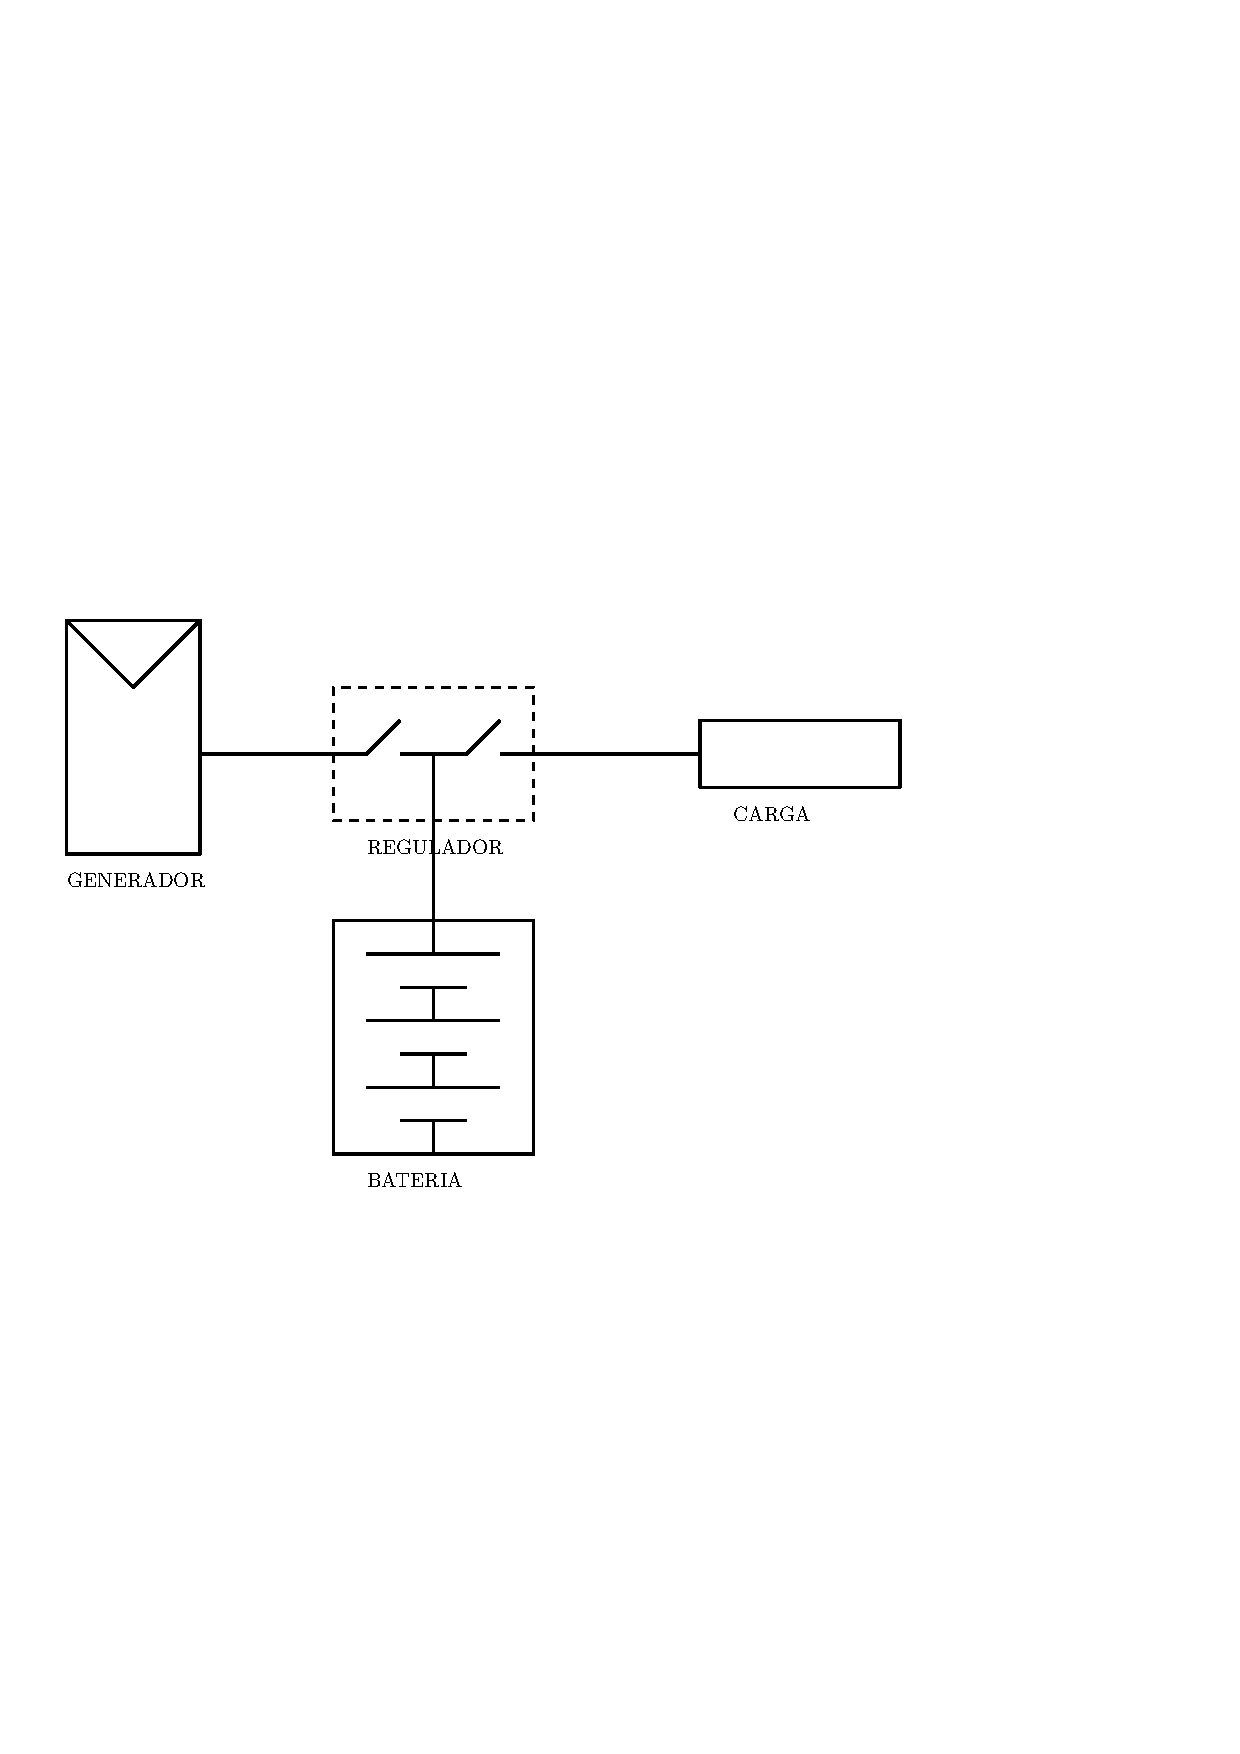
\includegraphics[scale=0.4]{../figs/DiagramaUnifilarER_DC}



}\hfill{}\subfloat[AC.]{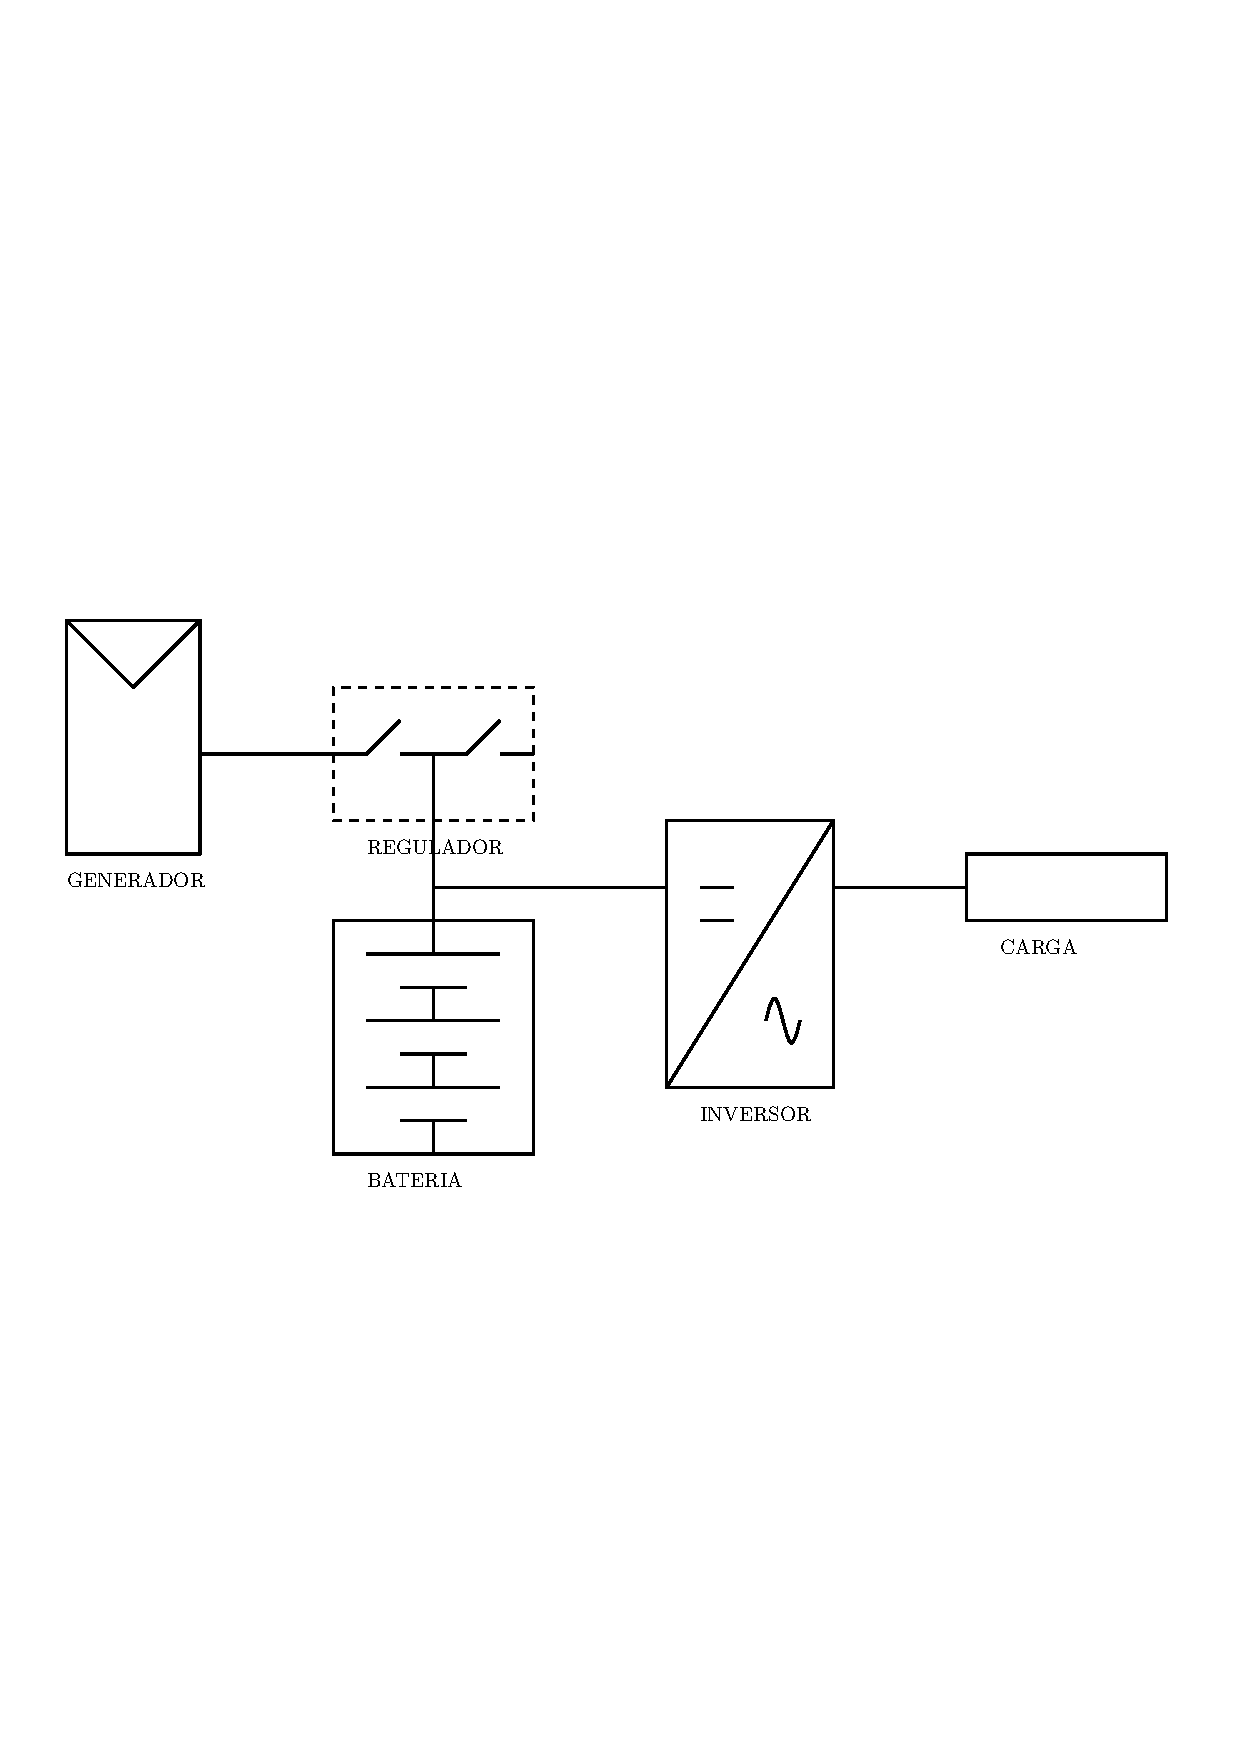
\includegraphics[scale=0.4]{../figs/DiagramaUnifilarER_AC}

}\hfill{}

\hfill{}\subfloat[AC-DC.]{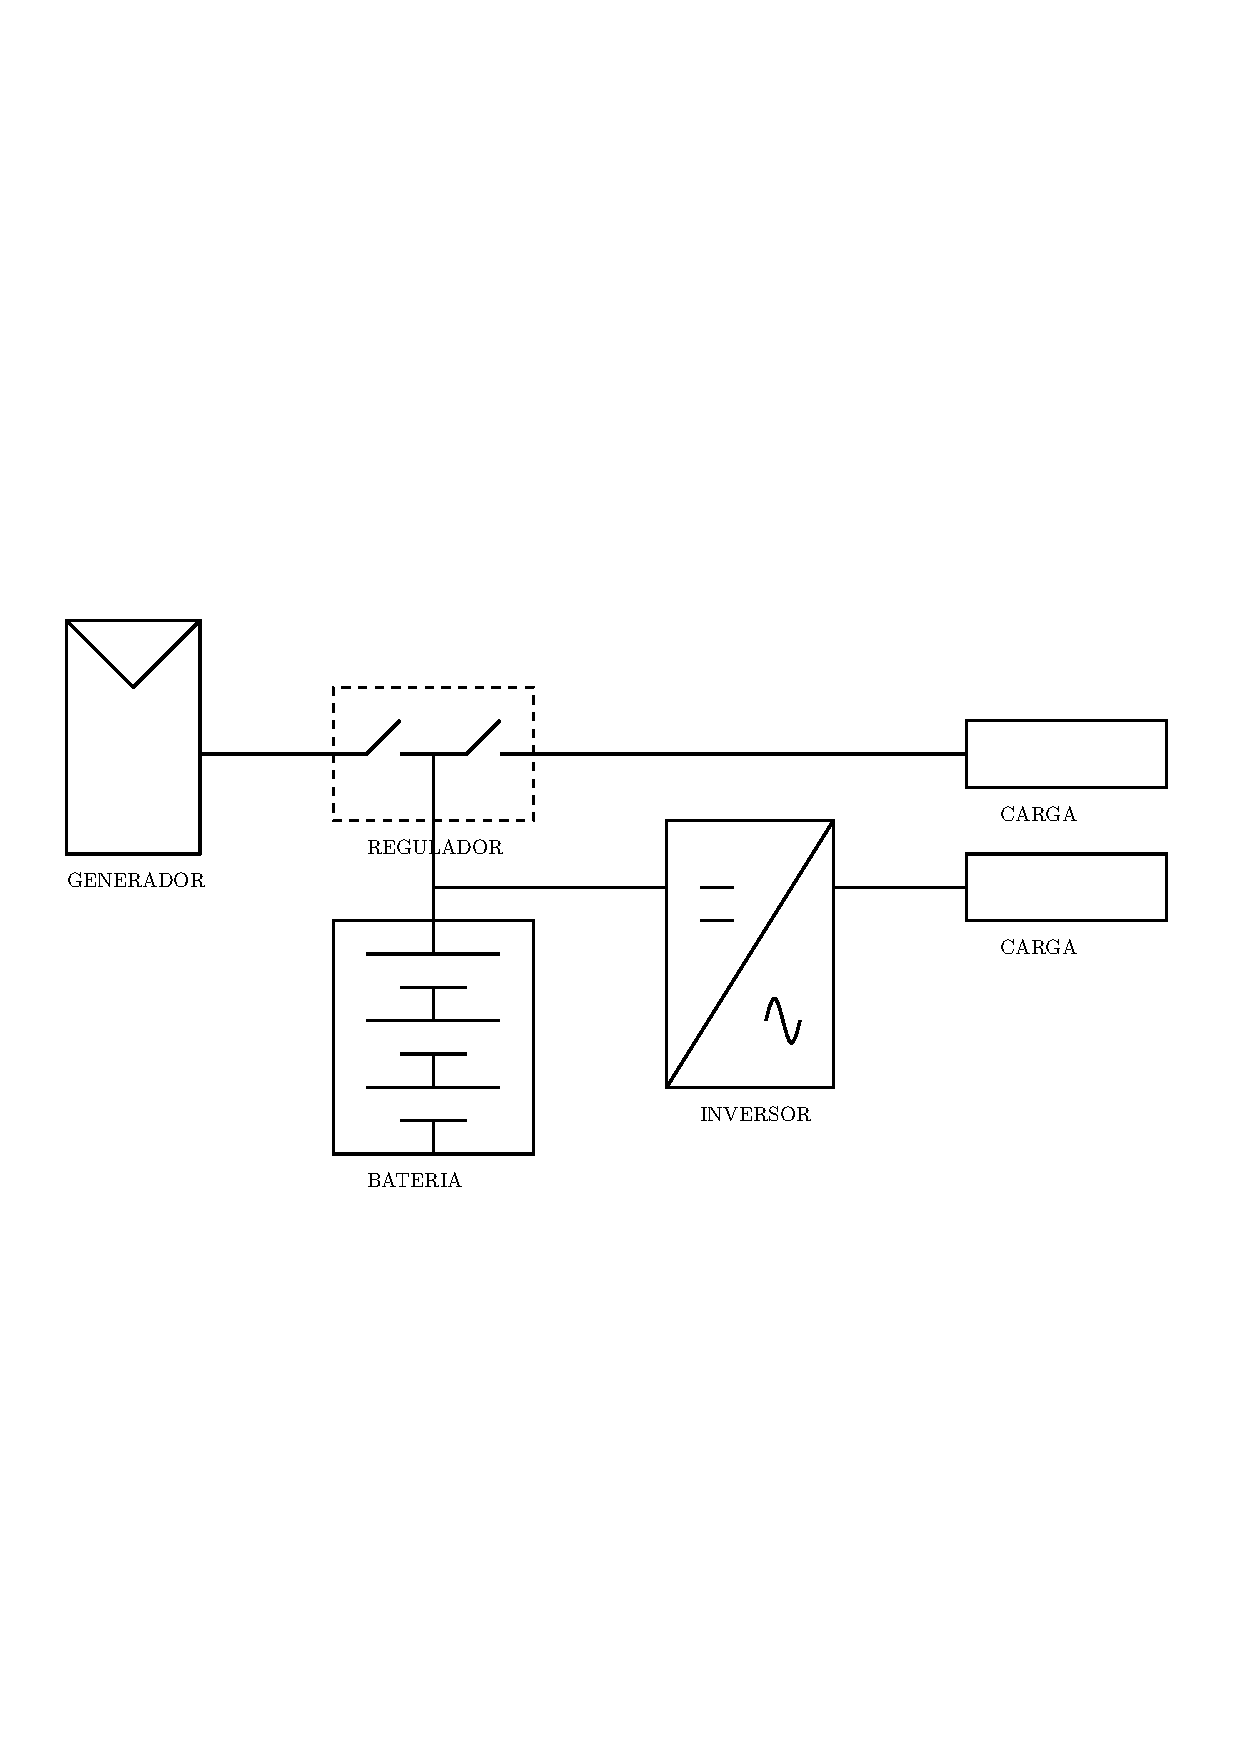
\includegraphics[scale=0.38]{../figs/DiagramaUnifilarER_AC_DC}

}\hfill{}\subfloat[Híbrido.]{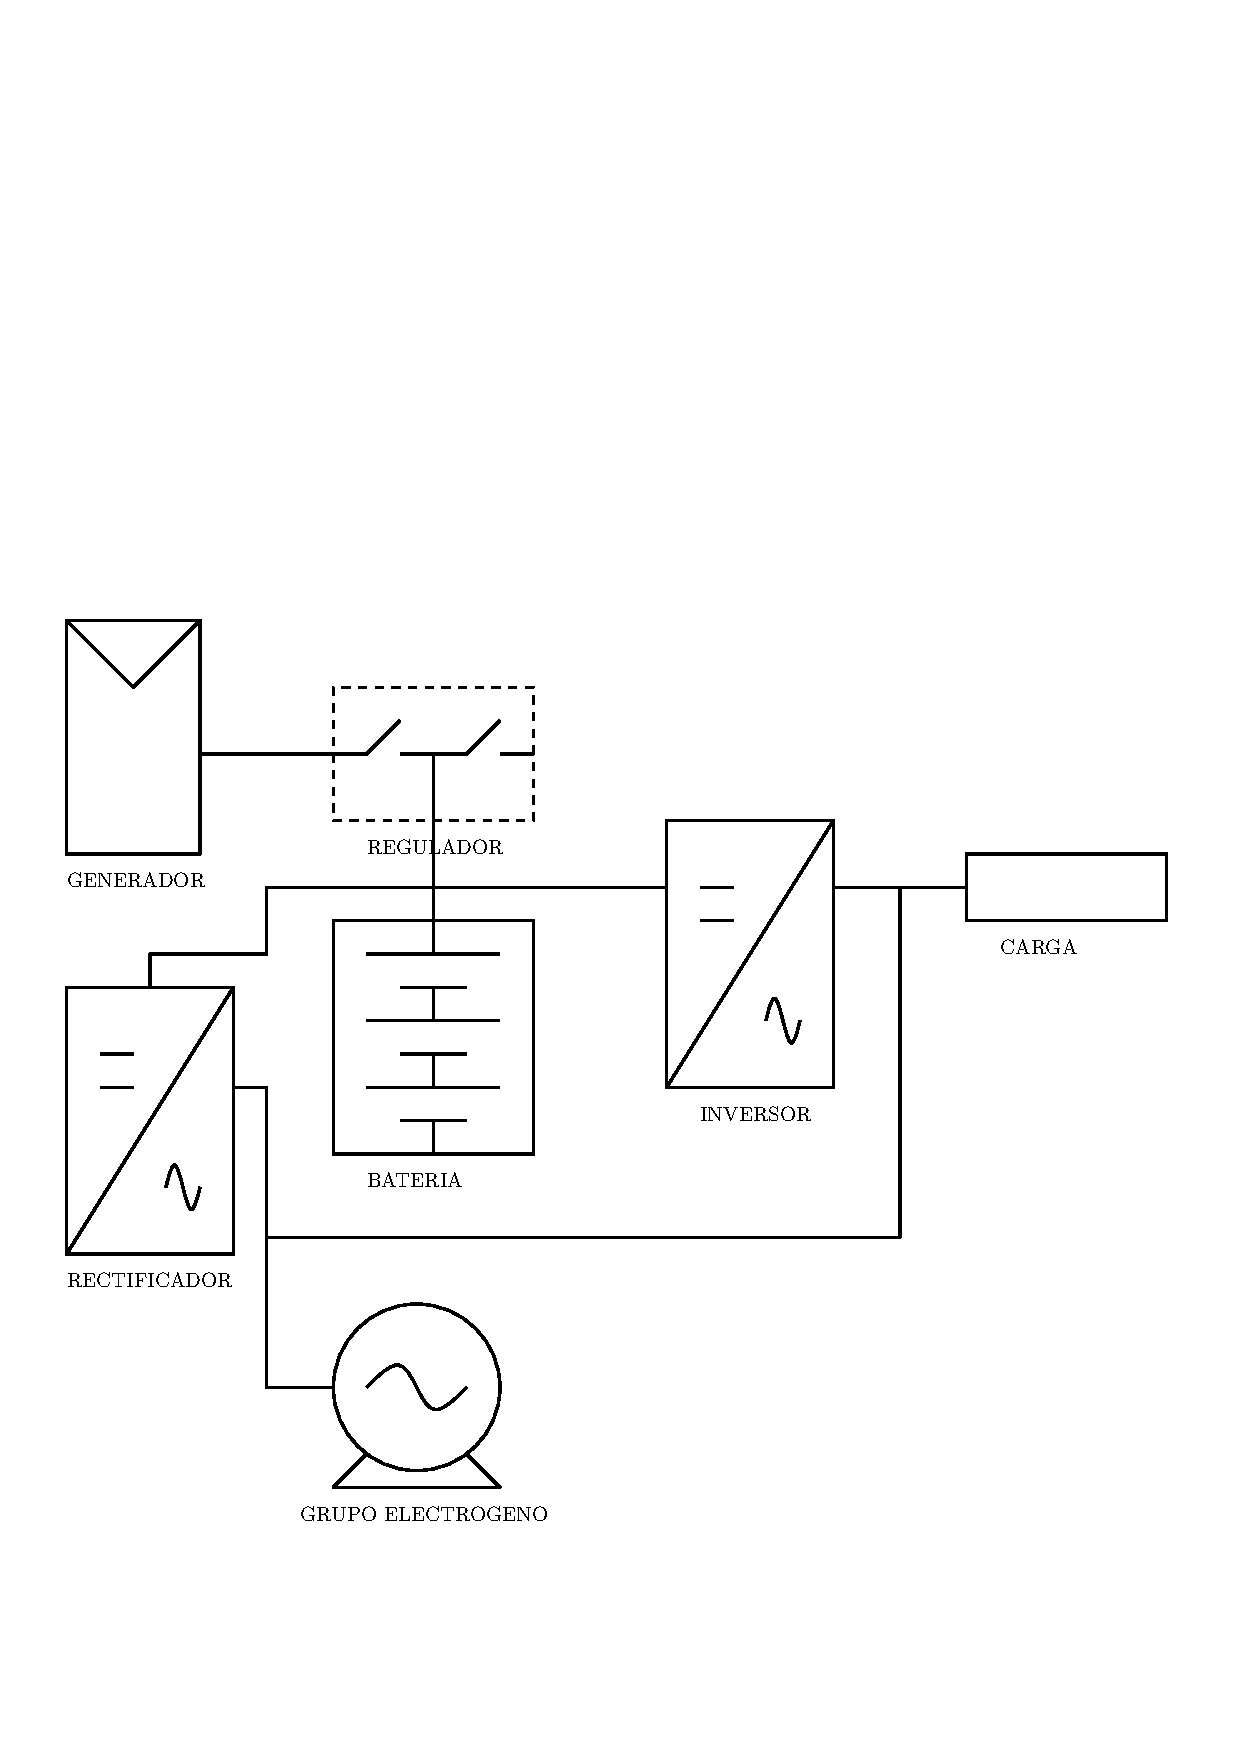
\includegraphics[scale=0.4]{../figs/DiagramaUnifilarER_Hibrido}

}\hfill{}

\caption{Configuraciones típicas.\label{fig:Configuraciones-tipicas_SFA}}



\end{figure}



\section{Componentes de un SFA}


\subsection{Acumulador electroquímico}

Un acumulador electroquímico es una batería secundaria o recargable,
capaz de almacenar energía eléctrica mediante una transformación en
energía electroquímica. Es capaz de dar autonomía al sistema fotovoltaico
al satisfacer los requerimientos de consumo en cualquier momento,
independientemente de la generación. También contribuye al buen funcionamiento
del sistema al aportar picos de intensidad superiores a los que proporciona
el generador FV y al estabilizar el voltaje del sistema, evitando
fluctuaciones dañinas en los equipos de consumo. 

La variada gama de acumuladores que se emplean en los SFA se basan,
casi en su totalidad, en la tecnología de ácido-plomo. Es por esta
razón que el contenido de este apartado hará referencia exclusiva
a este tipo de acumuladores.


\subsubsection{Definiciones}

Para comprender el desarrollo de este apartado se requieren unas definiciones
previas:
\begin{description}
\item [{Capacidad~nominal~($C_{b}$)}] es la carga eléctrica que puede
ser extraída de una batería hasta llegar a la descarga total.  \nomenclature[Cb]{$C_{b}$}{Capacidad nominal de un acumulador electroquímico}
\item [{Régimen~de~carga/descarga}] es la corriente aplicada a una batería
para restablecer/extraer la capacidad nominal. Normalmente se presenta
como un ratio entre la capacidad nominal y la corriente. Por ejemplo,
si la capacidad es 300 Ah, se habla de un régimen de carga (descarga)
$C_{10}$ cuando se aplican (extraen) 30 A, de forma que en 10 horas
se restablece (extrae) la capacidad. 

Habitualmente, la documentación técnica de los fabricantes incluye la
capacidad a $C_{10}$. Sin embargo, los regímenes de funcionamiento más
habituales en los sistemas fotovoltaicos son del orden de
$C_{100}$. Como regla aproximada puede emplearse la relación $C_{100}
\simeq 1.35 \cdot C_{10}$. Es importante resaltar que, debido a esta relación, la corriente $I_{10}$
correspondiente a $C_{100}$, no equivale a $0.1 \cdot I_{10}$. En el
caso anterior, con $C_{10}=\SI{300}{\ampere\hour}$,
$I_{10}=\SI{30}{\ampere}$, y como $C_{100}\simeq
\SI{405}{\ampere\hour}$, obtenemos $I_{100}=\SI{4.05}{\hour}$.
%OJO: capitulo de Sauer en Luque&Hegedus

% Para relacionar la capacidad a diferentes regímenes de carga es útil
% la ecuación experimental siguiente \cite{Copetti.Lorenzo.ea1993, Diaz.Lorenzo2001}:
% \begin{equation}
%   \label{eq:CxC20}
%   \frac{C_x}{C_{20}}=\frac{1.34}{1+0.34*(I_x/I_{20})^{0.9}}
% \end{equation}
% donde $I_x$ es la corriente correspondiente al régimen de carga $C_x$.
\item [{Estado~de~carga~(SoC)}] de una batería es la capacidad de una
batería parcialmente cargada, dividida por su capacidad nominal. Por
tanto siempre será $0<SoC<1$.\nomenclature[SoC]{SoC}{Estado de carga de un acumulador electroquímico}\nomenclature[PD]{PD}{Profundidad de carga de un acumulador electroquímico}
\item [{Profundidad~de~descarga~(PD)}] es el complemento del estado
de carga.
\item [{Tensión~de~corte:}] es la tensión a la que finaliza la descarga
de la batería. Depende del régimen de descarga y del tipo de batería.
Determina la profundidad de descarga máxima, $PD_{max}$, y por tanto,
la capacidad útil, $C_{U}$, siendo \begin{equation}
C_{U}=PD_{max}\cdot C_{b}\end{equation}
\nomenclature[PDmax]{$PD_{max}$}{Máxima profundidad de carga de un acumulador electroquímico}\nomenclature[Cu]{$C_{U}$}{Capacidad útil de un acumulador electroquímico}
\item [{Eficiencia~farádica}] es el ratio entre la carga extraída durante
la descarga y la carga requerida para restablecer el estado inicial.
\item [{Eficiencia~energética}] es el ratio entre la energía extraída
durante la descarga y la energía requerida para restablecer el estado
inicial.
\end{description}

\subsubsection{Funcionamiento}

Una batería de ácido-plomo se compone de un ánodo o electrodo positivo
con $\mathrm{PbO_{2}}$, un cátodo o electrodo negativo con Pb, y
el electrolito a base de $\mathrm{H_{2}SO_{4}}$ diluido en agua.
Su funcionamiento es una reacción electroquímica de oxidación-reducción:

Ánodo (+):\begin{equation}
\mathrm{PbO_{2}+SO_{4}^{2-}+H^{+}+2e^{-}
\xrightleftharpoons[\text{carga}]{\text{descarga}}
  PbSO_{4}+2H_{2}O}
\end{equation}


Cátodo (-):\begin{equation}
\mathrm{Pb+SO_{4}^{2-}
\xrightleftharpoons[\text{carga}]{\text{descarga}}
PbSO_{4}+2e^{-}}
\end{equation}


Global:\begin{equation}
\mathrm{Pb+PbO_{2}+2H_{2}SO_{4}
\xrightleftharpoons[\text{carga}]{\text{descarga}}
2PbSO_{4}+2H_{2}O}
\end{equation}


Durante la descarga, ambos electrodos transforman la materia activa
en sulfato de plomo y con agua en el ánodo. Este proceso supone consumo
de electrolito (disminuye su densidad) y cambios de volumen de los
materiales activos (el volumen del $\mathrm{PbSO_{4}}$ es superior
al del $\mathrm{PbO_{2}}$ y este al del $\mathrm{Pb}$). Dado que
las reacciones químicas se producen en la superficie porosa de la
materia activa, los cambios de volumen dificultan la homogeneidad
del proceso y la adecuada difusión del electrolito entre la materia
activa. Más aún, la concatenación de cambios de volumen provoca tensiones
mecánicas en las rejillas con la consiguiente fractura del material
activo que se desprende y precipita al fondo. Como consecuencia, las
descargas repetidas producen pérdida de material activo y degradación
de las placas. Por otra parte, si la descarga es muy rápida y la batería
permanece descargada largo tiempo, el sulfato cristaliza y no es recuperable.
A este fenómeno se le denomina sulfatación. 

Durante la carga, el sulfato de plomo se transforma en oxido de plomo,
plomo y ácido. Cuando el proceso de carga está por finalizar, la reacción
química implica la electrolisis del agua, con liberación de oxigeno
e hidrógeno (conocido como gaseo). Esta liberación supone la pérdida
de agua del electrolito pero también la homogeneización del electrolito
por agitación. Este fenómeno reduce la estratificación del electrolito,
situación que se produce cuando la gravedad y la falta de movimiento
provocan mayor concentración de electrolito en la zona inferior, pero
también contribuye a la corrosión por oxidación de la rejilla positiva,
por lo que su utilización debe ser controlada convenientemente. Más
aun, debe tenerse en cuenta que la pérdida de agua producida por el
gaseo debe ser compensada en el proceso de mantenimiento. 

Una alternativa para evitar la reposición de agua es el tipo de baterías
VRLA (\emph{valve-regulated lead acid}). Utilizan recipientes sellados
con una válvula que permite la liberación de gas sólo cuando la presión
en el interior sobrepasa un umbral (fenómeno producido por una sobrecarga
excesiva, que debe ser evitado en este tipo de baterías). En condiciones
normales de funcionamiento, el gas queda confinado en la batería y
se recombina para producir nuevamente agua. Estas baterías inmovilizan
el electrolito, que ya no está en fase líquida. Existen dos métodos
a destacar: las baterías de gel (añaden $\mathrm{SiO_{2}}$ al electrolito)
y las baterías AGM (\emph{absorbed glass matt}) en las que el electrolito
es absorbido en un conjunto de fibras de cristal con alta porosidad. 


\paragraph{Modelo eléctrico}

Una batería de ácido-plomo puede ser modelada como una fuente de tensión,
$V_{BI}$, en serie con una resistencia, $R_{BI}$, tal y como se
indica en la Figura \ref{fig:Modelo-de-bateria}.\nomenclature[Vbi]{$V_{BI}$}{Tensión en circuito abierto de una batería}\nomenclature[Rbi]{$R_{BI}$}{Resistencia interna de una batería}
Como será estudiado a continuación, ambos parámetros están relacionados
con la densidad del electrolito y con la temperatura. Un incremento
en la concentración del ácido provoca un aumento en $V_{BI}$ y una
disminución en $R_{BI}$, ya que las reacciones se producen más fácilmente.
Por el contrario, con la disminución de la densidad $V_{BI}$ disminuye
y $R_{BI}$ aumenta. 

%
\begin{figure}
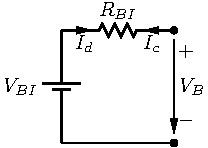
\includegraphics{../figs/Bateria}

\caption{Modelo eléctrico de batería.\label{fig:Modelo-de-bateria}}

\end{figure}


Con este modelo, la tensión de salida de la batería en el proceso
de carga es el descrito por la ecuación \ref{eq:TensionBateriaCarga}. 

\begin{equation}
V_{B}=V_{BI}+I_{C}R_{BI}\label{eq:TensionBateriaCarga}\end{equation}
mientras que en el proceso de descarga es (ecuación \ref{eq:TensionBateriaDescarga}):

\begin{equation}
V_{B}=V_{BI}-I_{D}R_{BI}\label{eq:TensionBateriaDescarga}\end{equation}
\nomenclature[Vb]{$V_{B}$}{Tensión en funcionamiento de una batería}\nomenclature[Id]{$I_{D}$}{Corriente de descarga de un acumulador electroquímico}\nomenclature[Ic]{$I_{C}$}{Corriente de carga de un acumulador electroquímico}

El comportamiento de la fuente de tensión equivalente está relacionado
directamente con la densidad de electrolito. Cuando el electrolito
es homogéneo, es posible aplicar la ecuación \ref{eq:TensionBateriaDensidad}:

\begin{equation}
V_{BI}=\rho_{e}+0.84\label{eq:TensionBateriaDensidad}\end{equation}
\nomenclature[rhoe]{$\rho_{e}$}{Densidad del electrolito de una batería de acido-plomo}

Para baterías cargadas, $\rho_{e}$ varia entre $\SI{1.2}{\gram\per\cm\cubed}$
y $\SI{1.28}{\gram\per\cm\cubed}$. Por tanto, la tensión en circuito
abierto de un vaso, $V_{BI}$, está comprendida entre $\SI{2.04}{\volt}$
a $\SI{2.12}{\volt}$. Precisamente la medida de la tensión en circuito
abierto de la batería es un método posible para estimar el estado
de carga de una batería, con el inconveniente de que una medida precisa
requiere desconectar el acumulador del sistema.

En la figura \ref{fig:CurvasCarga} se muestra la evolución de la
tensión en bornes de una batería cargada con corriente constante a
lo largo del tiempo. Esta figura incluye varias curvas para diferentes
valores de corriente de carga y de temperatura ambiente. En cada una
de ellas pueden observarse tres zonas de comportamiento. La primera
de ellas, comprendida entre el inicio de carga y el primer punto de
inflexión es la zona de carga normal, en la que la producción de ácido
provoca el aumento de $V_{BI}$ y la disminución de $R_{BI}$. Dado
que el valor de $V_{BI}$ en esta zona es superior al producto $I_{C}\cdot R_{BI}$,
es evidente el consiguiente aumento de $V_{B}$. La segunda zona a
diferenciar está comprendida entre los dos puntos de inflexión. El
primer punto de inflexión corresponde al inicio del gaseo, y el segundo
corresponde a la tensión de final de carga. En esta segunda zona se
produce la electrólisis del agua (gaseo) que se corresponde con un
incremento notable de la resistencia $R_{BI}$, debido a que el proceso
se realiza con más dificultad%
\footnote{En esta zona, el rendimiento farádico empieza a decrecer, lo que indica
que la corriente entrante no se emplea en el almacenamiento de energía
sino en procesos secundarios. De ahí que esta corriente entrante no
será directamente aprovechable en el proceso de descarga.%
}. A partir del segundo punto de inflexión la tensión se mantiene constante.
Adentrarse en esta zona de trabajo implica la degradación de la batería,
y por tanto, debe ser evitada.

Dado que la gasificación por sobrecarga, útil para reducir la estratificación,
debe ser un proceso controlado para evitar acortar la vida de la batería,
es necesario establecer un límite de carga en la batería. Como se
detalla en el siguiente apartado, en los equipos reguladores es práctica
común utilizar la tensión del vaso como indicador indirecto del estado
de carga, y por tanto, este límite vendrá definido por un valor de
tensión. Como puede observarse en la figura \ref{fig:CurvasCarga},
estos límites varían con la corriente de carga y con la temperatura.
Para una temperatura de $\SI{25}{\celsius}$ parece razonable utilizar
un valor comprendido entre $\SI{2.3}{\volt}$ y $\SI{2.4}{\volt}$,
tal y como se indica en la Norma Técnica Universal para Sistemas Fotovoltaicos
Domésticos \citep{Egido.Lorenzo1998}.

%
\begin{figure}
\begin{centering}
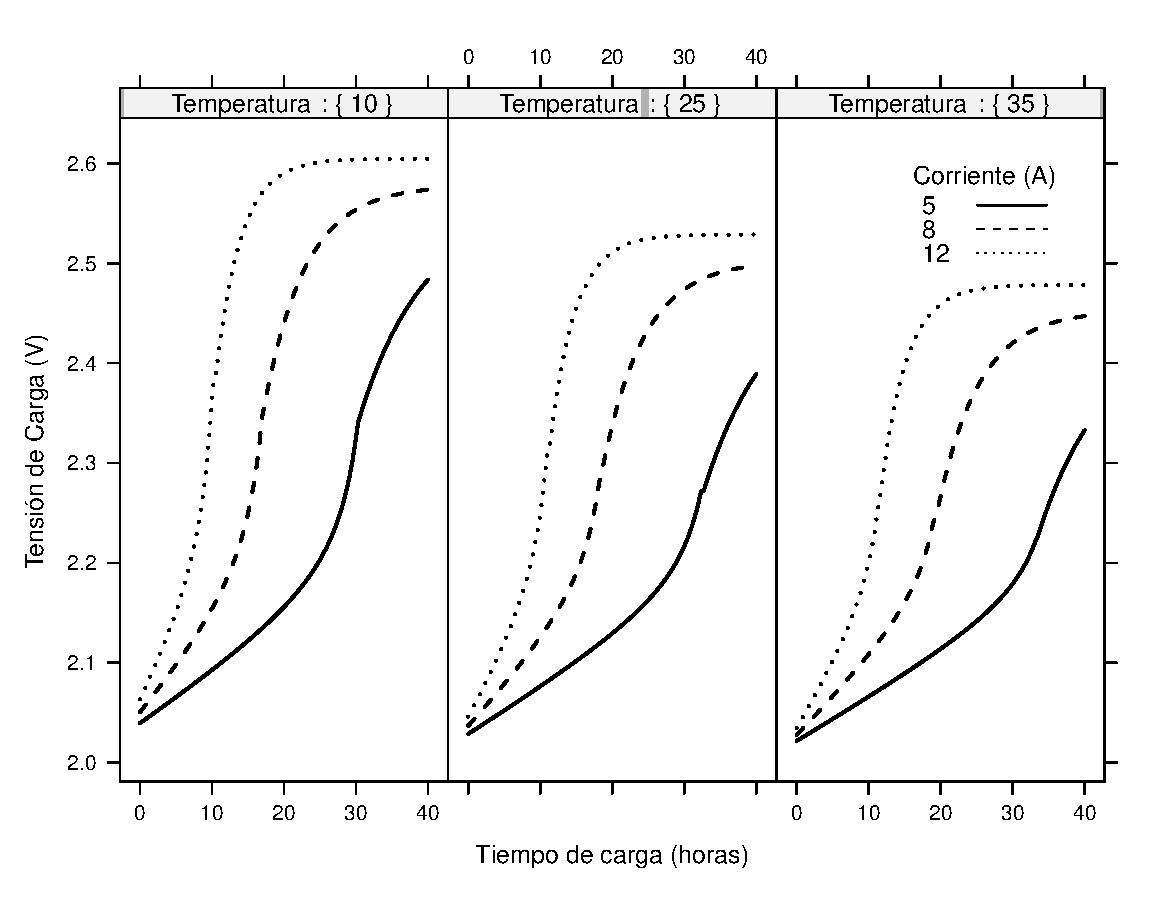
\includegraphics[scale=0.75]{../figs/Bateria_CorrYTemp}
\end{centering}

\caption[Curvas de evolución de la tensión en bornes de una batería durante
un proceso de carga a corriente constante]{Curvas de evolución de la tensión en bornes de una batería durante
un proceso de carga a corriente constante, para diferentes valores
de corriente de carga y temperatura ambiente. Las curvas están particularizadas
para una batería con una capacidad $C_{10}=\SI{300}{Ah}$. Se ha utilizado
el modelo de comportamiento propuesto en la referencia \citep{Copetti.Lorenzo.ea1993}.\label{fig:CurvasCarga}}

\end{figure}


Durante la descarga, la tensión $V_{BI}$ disminuye y la resistencia
$R_{BI}$ aumenta, de forma que la tensión en bornes de la batería,
$V_{B}$, disminuye durante el proceso. En la figura \ref{fig:CurvaDescarga}
se observa que la tensión en bornes de la batería evoluciona de forma
lineal durante todo el proceso, decreciendo abruptamente al acercarse
a la descarga total. Si nuevamente recurrimos a la tensión como indicador
del estado de carga de la batería, el equipo regulador deberá evitar
la descarga de la batería a partir de un umbral localizado en torno
a los $\SI{2}{\volt}$ para esta batería concreta. Tal y como se indica
en \citep{Egido.Lorenzo1998}, este valor es característico de cada
tipo de batería, y por tanto deben evitarse valores universales.

%
\begin{figure}
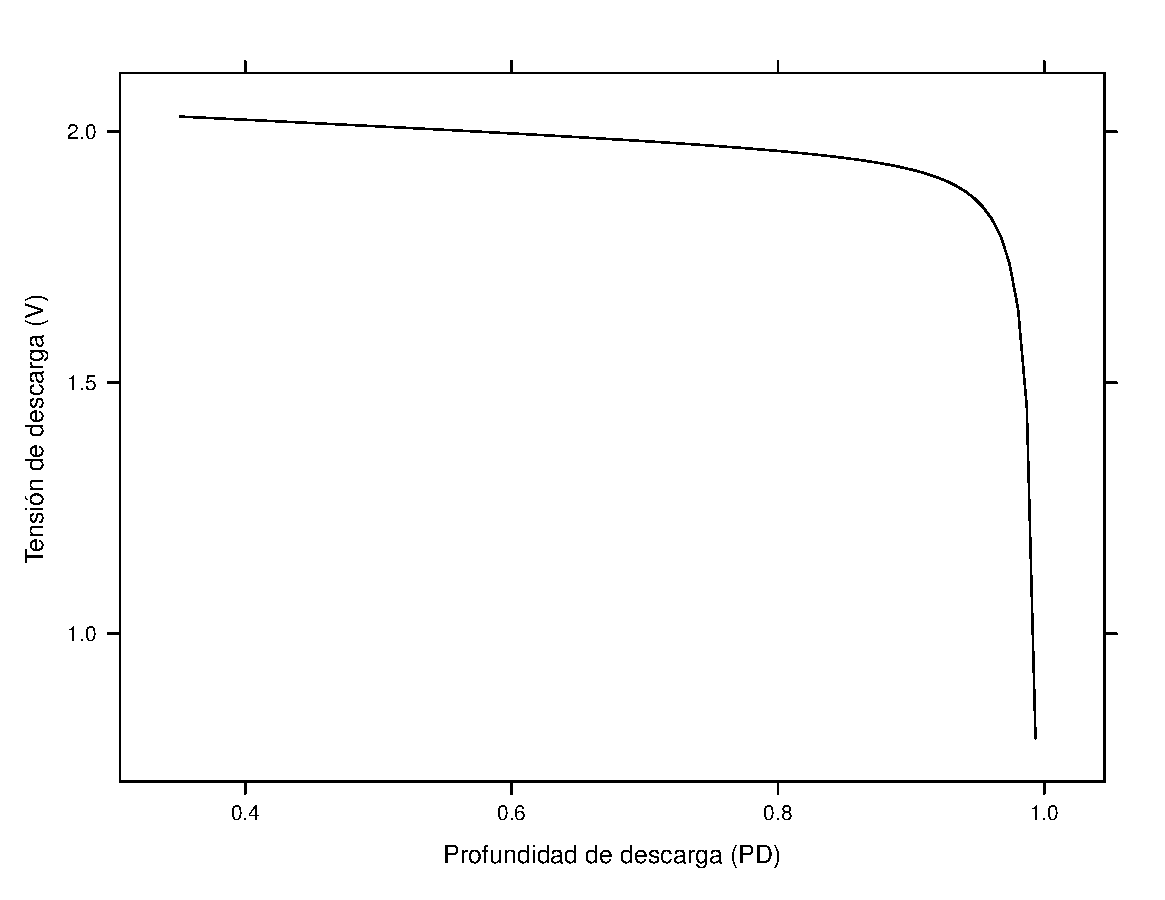
\includegraphics[scale=0.6]{../figs/Bateria_SOCyDescarga}

\caption[Relación entre la tensión y la profundidad de descarga de una batería
para un proceso de descarga a corriente constante]{\label{fig:CurvaDescarga}Relación entre la tensión y la profundidad
de descarga de una batería para un proceso de descarga a corriente
constante. Esta curva está particularizada para un régimen de descarga
de 100 h y temperatura ambiente de $\SI{25}{\celsius}$, para una
batería con capacidad $C_{10}=\SI{300}{Ah}$.}



\end{figure}


El régimen al que se produce la descarga está relacionado con la capacidad
que presenta la batería. Así, la mayor capacidad está disponible para
regímenes de carga lentos, tal y como se puede observar en la figura
\ref{fig:RegimenDescargaCapacidad}.

%
\begin{figure}
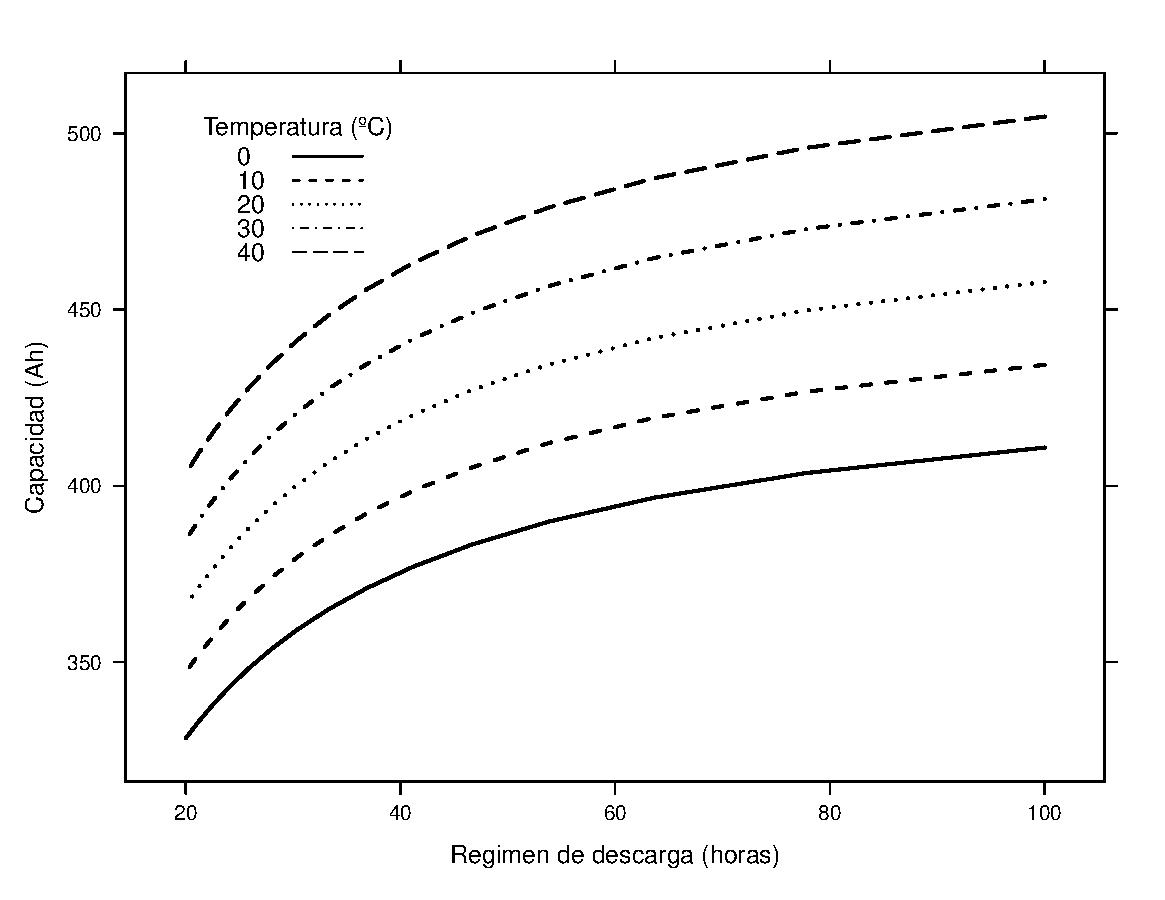
\includegraphics[scale=0.75]{../figs/Bateria_Capacidad}

\caption{Relación entre el régimen de descarga y la capacidad de la batería.\label{fig:RegimenDescargaCapacidad}}



\end{figure}



\paragraph{Efecto de la temperatura}

Cuando la temperatura ambiente es baja, el electrolito se hace más
viscoso y decrece la movilidad de los iones, aumentando así la resistencia
eléctrica ($R_{BI}$ en el modelo). La figura \ref{fig:RegimenDescargaCapacidad}
muestra que la la disminución de la temperatura reduce la capacidad
de la batería para todos los regímenes de descarga. De forma aproximada,
puede decirse que la capacidad para un régimen de descarga determinado
baja a razón de $\SI{1}{\percent\per\celsius}$ \citep{Lorenzo1994}.
Como situación extrema, si el electrolito se congela, no hay movimiento
iónico, y por tanto la capacidad es nula. Para evitarlo, en lugares
muy fríos hay que recurrir a densidades altas de electrolito .

Cuando la temperatura ambiente es alta, las reacciones se aceleran
($R_{BI}$ disminuye), y la corrosión se ve favorecida, siendo éste
un factor de degradación de las baterías. Así, en climas cálidos,
se debe optar por bajas concentraciones de electrolito. Esta elección
aumenta la resistencia equivalente, pero este hecho se ve compensado
por la mayor movilidad iónica debida a la alta temperatura.

Tal y como se observa en la figura \ref{fig:CurvasCarga}, hay que
tener en cuenta que el valor de tensión al que empieza la sobrecarga
disminuye debido a que la resistencia interna baja con la temperatura.
Por tanto, es necesario corregir el umbral de corte con la temperatura.
Dado que las corrientes que circulan por la batería son de un valor
tal que no incrementan significativamente la temperatura de la batería
respecto de la ambiente, es aceptable utilizar ésta como referencia
para la corrección.


\subsubsection{Ciclado. Mecanismos de degradación}

A lo largo de su operación, la batería es sometida a continuas cargas
y descargas. Este proceso se denomina ciclado, y según sus características
tendrá unas consecuencias determinadas sobre la vida de la batería.
Los dos mecanismos de degradación principales asociados al ciclado
son la perdida de material activo que ocasionan las descargas repetidas,
y la estratificación. 

La estratificación se produce por la acción conjunta de la resistencia
de las rejillas, la falta de movimiento de la batería y la gravedad.
Así, cuando se produce la descarga de una batería inicialmente
cargada, la resistencia de las rejillas provocará que la densidad de
corriente de las zonas superiores sea mayor que en las zonas
inferiores.  Por tanto, al finalizar la descarga, el perfil de
densidad del electrólito no será uniforme en toda la altura de la
batería, sino que mostrará un máximo en la parte baja. Cuando, a
continuación, se inicia una carga, la densidad de corriente en la zona
inferior de las rejillas será superior dado que la mayor densidad de
electrolito es sinónimo de menor resistencia eléctrica interna
($R_{BI}$). De esta forma, el proceso de estratificación iniciado en
la descarga se reafirma en la carga posterior. El efecto de la
gravedad y la ausencia de movimiento%
\footnote{Por ejemplo, las baterías instaladas en vehículos raramente
  están estratificadas, porque el propio movimiento de estos
  homogeneiza el electrolito.%
} en la batería contribuirán a agravar este desequilibrio, de forma
que la mayor densidad del electrolito sobre el agua provocará que
aquel se desplace hacia el fondo. El alto nivel de concentración de
ácido en las zonas inferiores consecuencia de la estratificación
contribuye a la corrosión de las rejillas. En estas condiciones es
conveniente recurrir al gaseo que se produce durante una sobrecarga
controlada, útil para remover el electrolito y homogeneizarlo.

Existen otros mecanismos de degradación. Destacan los siguientes:
\begin{itemize}
\item Corrosión\textbf{\emph{ }}externa\textbf{ }de los terminales: Aumenta
la resistencia de contacto, de forma que la corriente no se distribuye
uniformemente entre los vasos que componen un conjunto acumulador.
Se produce en ambientes agresivos y con altas temperaturas, siendo
recomendable la aplicación de grasas y limpieza en los terminales
de conexión.
\item Corrosión interna de las rejillas: Durante la sobrecarga, el material
de las rejillas se degrada, formando depósitos en los vasos. Este
fenómeno disminuye la capacidad de forma irreversible.
\item Gaseo excesivo: Cuando se permite una sobrecarga excesiva para eliminar
la estratificación, el gaseo produce pérdidas de electrolito, corrosión
en la placa positiva y averías en las baterías VRLA.
\item Sulfatación: Cuando la batería opera en largos periodos de carga parcial
el sulfato de plomo cristaliza, y deja de participar en las reacciones
químicas, disminuyendo así la capacidad de forma irreversible. Además,
al cristalizar se produce un cambio de volumen local, provocando tensiones
en la rejilla que pueden ocasionar fisuras.
\item Depósitos de materia activa: cuando la batería opera en bajos estados
de carga durante largos periodos, la materia activa pierde adherencia
y puede precipitar al fondo del vaso. Además de disminuir la capacidad,
puede ocasionar cortocircuitos que causen la muerte de la batería.
\end{itemize}
Como resumen, los factores que influyen sobre la resistencia del acumulador
al ciclado son \citep{Fullea1994}:
\needspace{3\onelineskip}
\begin{itemize}
\item La profundidad de descarga: las descargas profundas disminuyen los
ciclos de vida de una batería.
\item El régimen de carga: cuanto mayor es el régimen de carga y el porcentaje
de sobrecarga, menor será la vida alcanzada.
\item La temperatura: las temperaturas altas aceleran la corrosión en los
electrodos disminuyendo los ciclos de vida.
\end{itemize}
El ciclado y los agentes externos contribuyen a degradar el acumulador
hasta que alcanza el fin de su vida útil, momento que puede ser definido
como un valor mínimo en su capacidad útil \citep{Egido.Lorenzo1998}.


\subsubsection{Composición}

%
\begin{figure}
\begin{centering}
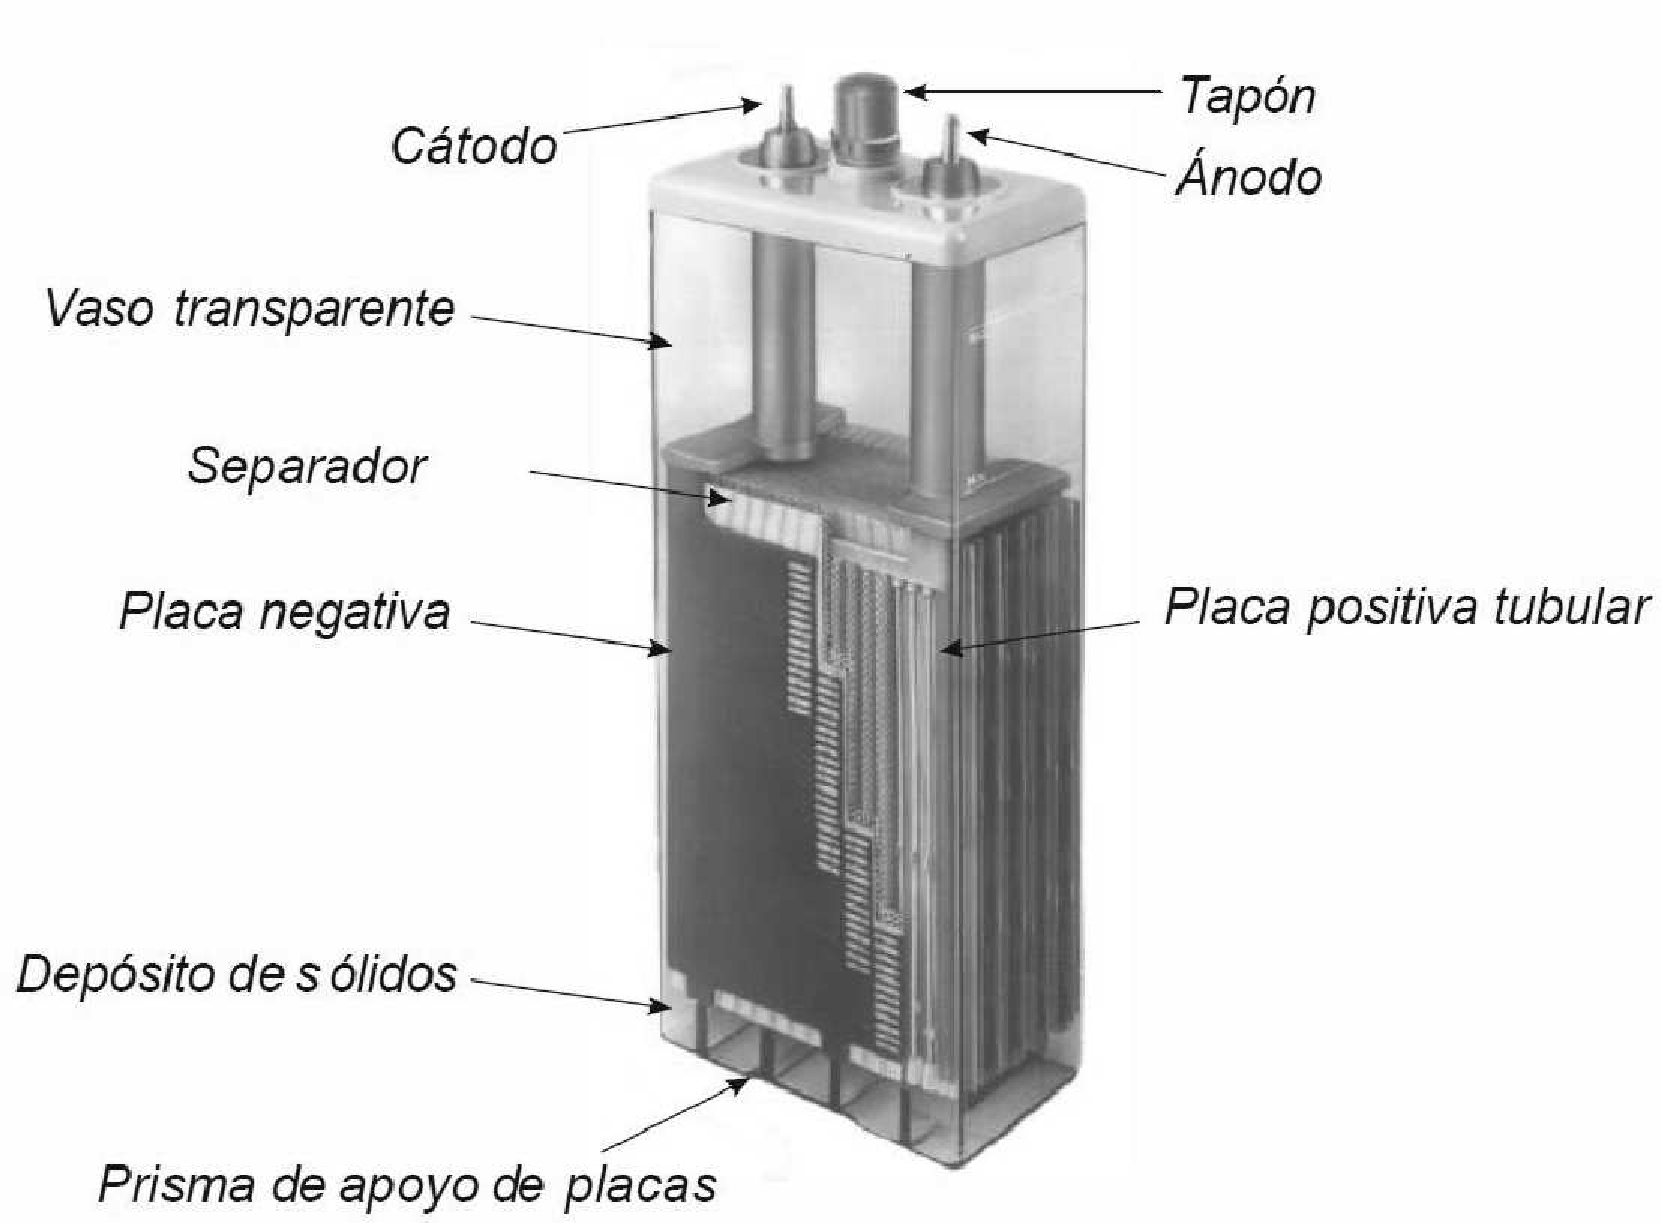
\includegraphics[scale=0.4]{../figs/AcumuladorBN}
\end{centering}

\caption{Batería estacionaria con desglose de elementos.\label{fig:Bateria-estacionaria}}

\end{figure}


Los elementos típicos de una batería quedan señalados en la figura
\ref{fig:Bateria-estacionaria}. Las rejillas dan soporte estructural
a los materiales activos (oxido de plomo en ánodo, plomo en cátodo)
y conducen la corriente eléctrica hacia el circuito externo. Están
fabricadas en aleaciones de plomo. La aleación de plomo-calcio proporciona
alta resistencia a la corrosión por sobrecarga pero presenta elevada
corrosión en bajos estados de carga, mientras que la aleación de plomo-antimonio
presenta buen comportamiento en ciclado y en descarga profunda. La
rejilla negativa es plana, mientras que la rejilla positiva puede
ser plana (para operación en flotación) o tubular (para operación
en ciclado).

Los materiales activos participan en las reacciones químicas. Están
adheridos a las rejillas. Deben ser porosos para permitir la penetración
del electrolito.

El electrolito participa en la reacción y realiza el transporte iónico
para cerrar el ciclo de corriente de las reacciones. La elección del
electrolito debe tener en cuenta su densidad, conductividad, punto
de congelación, poder de corrosión e impurezas. Para reducir la resistencia
eléctrica del electrolito, su densidad debe ser alta, pero un electrolito
de alta densidad es muy agresivo (produce corrosión en la rejilla
positiva). Por otra parte, altos regímenes de descarga requieren mayor
densidad para facilitar el transporte iónico. Los acumuladores estacionarios
utilizan densidades más bajas que los de arranque. El electrolito
puede ser líquido (aireadas) o inmovilizado (VRLA).

Los separadores aislan las placas de diferente polaridad pero permiten
el movimiento iónico a través suyo. Deben tener resistencia mecánica,
ser permeables y porosas, resistentes a la oxidación, sin contaminantes
y eléctricamente no conductores.




\subsubsection{Tipos de acumuladores}

Un acumulador incorporado a un SFA debe ser capaz de funcionar sometido
a ciclados diarios y anuales de carga y descarga, teniendo en cuenta
que la carga entregada por el generador depende directamente de la
radiación (variable en los períodos intradiario e intraanual). Debido
a las posibles fluctuaciones en la carga aportada, es probable que
se sucedan periodos prolongados en carga parcial. Por último, dadas
las características del consumo conectado a los SFA, es habitual que
las descargas sean a baja intensidad con periodos de descarga largos,
típicamente en torno a las 100 horas.

Existen cuatro tipos de acumuladores que son de interés en los sistemas
fotovoltaicos autónomos, todos basados en la tecnología de ácido-plomo.

Los más sencillos son las denominadas \textbf{baterías de arranque}
(\emph{SLI: Starting, Lighting, Ignition}), habitualmente empleadas
en automóviles, y por tanto fácilmente localizables en cualquier mercado
local. Esta característica junto a su bajo precio (comparado con otras
opciones) las convierten en una opción frecuentemente empleada en
sistemas de electrificación rural de pequeño tamaño, y suelen utilizarse
como reemplazo de baterías estropeadas si el servicio de mantenimiento
no funciona correctamente. Presentan un buen comportamiento en descarga
de alta intensidad y tienen buen rendimiento de descarga a bajas temperaturas.
Sin embargo, no son resistentes frente al ciclado, con lo que su vida
útil se acorta sustancialmente al funcionar en un sistema fotovoltaico.

En segundo lugar cabe mencionar las \textbf{baterías de tracción}
(empleadas, por ejemplo, en carretillas elevadoras). Por razón de
su aplicación tienen resistencia suficiente para soportar un elevado
número de ciclos profundos de carga-descarga. Como contrapartida,
requieren aportación de agua y mantenimiento frecuente. Por esta razón,
su empleo en sistemas fotovoltaicos autónomos sólo es aconsejable
cuando exista la seguridad de que el usuario y el servicio de mantenimiento
cuidarán este elemento de forma regular.

A continuación destacan las denominadas \textbf{baterías estacionarias}
(figura \ref{fig:Bateria-estacionaria}), comúnmente empleadas
en sistemas de alimentación ininterrumpida (UPS) o instalaciones remotas
(por ejemplo, radioenlaces). Habitualmente funcionan en régimen de
flotación (salvo casos esporádicos, no deben entregar carga). Este
modo de funcionamiento obliga a que posean gran reserva de electrolito
aunque realizan poco uso de agua. Son baterías con resistencia a la
corrosión y elevada fiabilidad. Todas estas características las convierten
en una opción muy interesante para su incorporación a los SFA. No
obstante, debe tenerse en cuenta su precio más elevado frente a las
anteriores opciones.

Finalmente, señalemos las denominadas \textbf{baterías {}``fotovoltaicas''}.
En el segmento económico de este tipo de baterías es posible encontrar
baterías SLI modificadas para adaptarse a las condiciones de funcionamiento
de un SFA, mientras que en el segmento alto se ofrecen baterías estacionarias
modificadas.

La elección entre uno u otro tipo es un ejercicio que debe tener en
consideración no sólo criterios puramente técnicos sino también aspectos
como el coste del sistema, recursos de mantenimiento disponibles durante
la vida del sistema, disponibilidad de reemplazo en el mercado local
o capacidad de intervención del usuario. No obstante, para aplicaciones
fotovoltaicas se recomienda usar baterías estacionarias aireadas de
placa positiva tubular, o al menos baterías SLI modificadas (placas
más gruesas, mayor cantidad de electrolito por encima de las placas,
más baratas que las estacionarias), con aleación de Pb-Sb en la rejilla
y vaso transparente \citep{Egido.Lorenzo1998}.


\subsection{Regulador de carga}

Un regulador de carga es un equipo electrónico capaz de evitar la
sobrecarga y la descarga excesiva de un acumulador cuando se alcanzan
determinados umbrales, generalmente determinados por la tensión en
bornes de la batería. 

Para proteger frente a la sobrecarga, el regulador puede desconectar
al generador de la batería (regulador serie, figura \ref{fig:ReguladorSerie})
o bien derivar la corriente del generador hacia otro lugar, sea este
un cortocircuito o un disipador (regulador \emph{shunt} o paralelo,
figura \ref{fig:ReguladorParalelo}). Esta última opción debe incorporar
un diodo de bloqueo entre el generador y la batería para evitar descargas
de ésta sobre el camino alternativo que ofrece el regulador. Para
proteger frente a la sobredescarga, lo común, tanto en reguladores
serie como paralelo, es desconectar los equipos de consumo de la batería.
Estos equipos suelen emplear interruptores MOSFETs como dispositivos
de conmutación.

Es conveniente observar que en las dos protecciones la batería siempre
es la que impone la tensión del sistema, sea al módulo, a los equipos
de consumo o al menos al regulador. Dicho de otra forma, los equipos
de consumo y el módulo nunca quedan conectados de forma directa sin
la intervención de la batería. Recordemos que una de las funciones
del acumulador es estabilizar la tensión del sistema y así evitar
fluctuaciones dañinas en los equipos de consumo.

%
\begin{figure}
\hfill{}\subfloat[Serie.\label{fig:ReguladorSerie}]{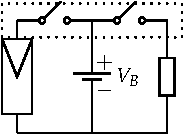
\includegraphics{../figs/ReguladorSerie}



}\hfill{}\subfloat[Paralelo.\label{fig:ReguladorParalelo}]{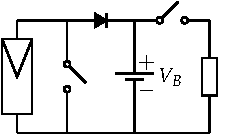
\includegraphics{../figs/ReguladorParalelo}



}\hfill{}

\caption{Esquema eléctrico de un regulador de carga.}



\end{figure}


El funcionamiento del regulador puede ser descrito por dos ciclos
de histéresis, uno para cada protección (figura \ref{fig:HisteresisRegulador}). 

%
\begin{figure}
\hfill{}\subfloat[\label{fig:HisteresisCarga}Carga]{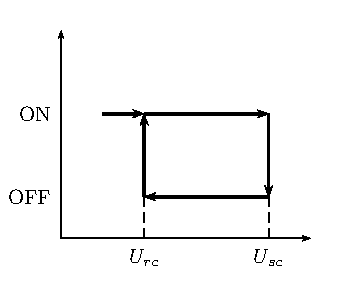
\includegraphics{../figs/HisteresisCargaRegulador}

}\hfill{}\subfloat[\label{fig:HisteresisDescarga}Descarga]{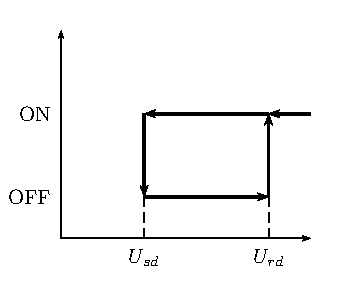
\includegraphics{../figs/HisteresisDescargaRegulador}}\hfill{}

\caption{\label{fig:HisteresisRegulador}Histéresis de protección frente a
sobrecarga y sobredescarga en un regulador.}

\end{figure}


En la protección contra la sobrecarga, el regulador dará orden de
desconexión del generador cuando la tensión de la batería supere el
{}``voltaje de fin de carga'', $U_{sc}$.\nomenclature[Usc]{$U_{sc}$}{Tensión de fin de carga en un regulador}
A partir de ese momento, la tensión de la batería, sometida ahora
a un proceso de descarga por los equipos de consumo, disminuirá su
tensión. Cuando ésta alcance el {}``voltaje de reposición'', $U_{rc}$\nomenclature[Urc]{$U_{rc}$}{Tensión de reposición de carga en un regulador},
comunicará de nuevo la batería con el generador. Hay dos tipos básicos
de estrategias de control. En los controladores {}``on-off'' se
interrumpe totalmente la corriente de carga cuando se alcanza el \textquotedblleft{}voltaje
de fin de carga\textquotedblright{}, mientras que en los controladores
con \textquotedbl{}modulación del ancho de pulso\textquotedbl{}, o
PWM, se recurre a reducir gradualmente la corriente de carga cuando
se alcanza el \textquotedblleft{}voltaje de fin de carga\textquotedblright{},
manteniendo así el voltaje constante, y precisamente igual a este
valor. Ambos tipos de reguladores y de estrategias de control son
adecuadas para SHSs sin que parezca existir una ventaja real asociada
a cada estrategia de control en términos de mejorar la vida útil de
la batería \citep{Egido.Lorenzo1998}. En la práctica la selección
de los voltajes de fin de carga y reposición debe buscar una solución
de compromiso que conjugue la carga completa de la batería (voltajes
altos) y evitar la corrosión de las rejillas y el excesivo consumo
de agua (voltajes bajos). Los umbrales deben adaptarse a cada tipo
de batería (mediante ensayos, o recomendaciones del fabricante). Sin
embargo, es importante notar que la sensibilidad del \textquotedblleft{}voltaje
de fin de carga\textquotedblright{} al tipo de batería es relativamente
baja y puede recurrirse a valores de uso general. El lector interesado
puede recurrir a la información incluida en las referencias \citep{Egido.Lorenzo1998,Usher.Ross1998}
que puede ser resumida en los siguientes puntos:
\begin{itemize}
\item En el caso de reguladores {}``on-off'' el \textquotedblleft{}voltaje
de fin de carga\textquotedblright{} debe estar en el rango de $\SI{2.3}{\volt}$
a $\SI{2.4}{\volt}$ por vaso a $\SI{25}{\celsius}$. En los reguladores
con control por modulación por ancho de pulso (PWM), la tensión constante
de fin de carga debe ser ligeramente inferior con el objetivo de reducir
la pérdida de agua y la tasa de corrosión, siendo el margen recomendado
de $\SI{2.3}{\volt}$ a $\SI{2.35}{\volt}$ por vaso a $\SI{25}{\celsius}$.
\item En los controladores \textquotedblleft{}on-off\textquotedblright{},
el voltaje de reposición debe estar en el rango de $\SI{2.15}{\volt}$
a $\SI{2.2}{\volt}$ por vaso a $\SI{25}{\celsius}$. 
\item El \textquotedblleft{}voltaje de fin de carga\textquotedblright{}
y el \textquotedblleft{}voltaje de reposición\textquotedblright{}
deben corregirse por temperatura a razón de $\SI{4}{\milli\volt\per\celsius}$
a $\SI{5}{\milli\volt\per\celsius}$ por vaso.
\end{itemize}
Para la protección contra la sobredescarga, el regulador desconecta
la batería de los equipos de consumo cuando la tensión alcanza el
umbral definido por $U_{sd}$.\nomenclature[Usd]{$U_{sd}$}{Tensión de corte de descarga en un regulador}
A partir de esta desconexión, la batería será sometida a un proceso
de carga por el generador fotovoltaico y su tensión subirá. Cuando
ésta alcance el valor de reconexión, $U_{rd}$\nomenclature[Urd]{$U_{rd}$}{Tensión de reposición de descarga en un regulador},
conecta de nuevo la batería a los equipos de consumo. En la práctica,
la selección del voltaje de desconexión debe buscar una solución de
compromiso entre un usuario satisfecho (valores bajos de desconexión
que maximizan la disponibilidad de energía) y la protección de la
batería y otros componentes del sistema (valores altos de desconexión
que alejan el riesgo de sobredescarga). Es conveniente el uso de avisos
luminosos en el regulador que alerten de la cercanía de la desconexión
para que el usuario pueda alterar la pauta de consumo y adaptarse
al funcionamiento del sistema. Existe una amplia variedad de combinaciones
de sistemas de alarma, siendo destacable el código de colores tipo
semáforo. Nuevamente, los voltajes de desconexión y reconexión de
carga deben adaptarse a cada tipo de batería. Sin embargo, a diferencia
de la protección contra sobrecarga, es preferible no recurrir a valores
universales para estos umbrales y es conveniente recurrir a las recomendaciones
del fabricante o ensayos en laboratorio para establecer los valores
adecuados. 


\subsection{Luminarias}

Las cargas típicas en los sistemas domésticos son luminarias, radios
y televisores, correspondiendo generalmente a la iluminación la parte
más importante del consumo energético. Por razones de eficiencia,
se recomienda el uso de lámparas fluorescentes.

Una lámpara fluorescente convencional está formada por un tubo de
descarga con gas a baja presión, un recubrimiento de una mezcla de
polvos fluorescentes y dos electrodos en los extremos. Aplicando tensión
entre los electrodos, debido a la ionización permanente del gas se
produce el movimiento de las partículas cargadas (corriente eléctrica).
La ionización permanente es producida por la radiación exterior, y
por tanto, es limitada. Alcanzado un umbral de tensión, la causa de
ionización cambia: la tensión aplicada supone un campo eléctrico suficiente
como para comunicar energía a los electrones, que ahora son capaces
de ionizar a los átomos del gas. Este proceso se realimenta y se produce
un efecto avalancha. A partir de esta etapa, con pequeños incrementos
de tensión la corriente aumenta rápidamente, hasta alcanzar un límite
que ocasiona un arco eléctrico, que debe ser controlado. Este arco
eléctrico afecta al gas, que emite energía electromagnética que es
absorbida por el material fluorescente para producir radiación en
el rango de lo visible. Al encender el tubo con picos de alta tensión,
se produce desgaste en los electrodos por el bombardeo iónico. Así,
el proceso de encendido es el que más contribuye a la degradación
de los tubos fluorescentes. Un método alternativo consiste en precalentar
los electrodos (con un circuito basado en un condensador y en una
resistencia) facilitando el paso a la etapa de emisión termoiónica,
y acortando el período de encendido. 

Es necesario el uso de un circuito auxiliar denominado balasto, capaz
de adecuar la tensión de entrada a la tensión de encendido necesaria
para que fluya corriente por el tubo, regular la corriente que circula
por el tubo una vez que se ha producido el encendido para evitar su
destrucción y precalentar los electrodos para reducir el impacto que
produce el proceso de encendido. 

La serie de encendidos y apagados repetidos degradan los componentes
del tubo recortando la vida de la lámpara. En la Norma Técnica Universal
\citep{Egido.Lorenzo1998} se recomienda que la lámpara resista un
mínimo de 10\,000 ciclos de encendido y apagado, y en todo caso,
deberá resistir 5\,000 ciclos. 

En las especificaciones técnicas de las lámparas fluorescentes se
emplean algunos conceptos de luminotecnia. Recogemos aquí los más
básicos y frecuentes:
\begin{itemize}
\item Flujo radiante: es la potencia emitida por la fuente luminosa (Unidad:
Watio).
\item Flujo luminoso: es la potencia emitida capaz de producir sensación
luminosa en el ojo humano (Unidad: Lumen).
\item Iluminación de una superficie sobre la que incide un flujo luminoso
es el ratio entre flujo y superficie (Unidad: lux, lumen/m\texttwosuperior{}).
\item Eficiencia de la luminaria (tubo y balasto) es la relación entre potencia
eléctrica consumida por el conjunto y la potencia luminosa producida
(Unidad: Lumen/Watio). Se recomienda que esta eficiencia sea superior
a $\SI{50}{\lumen\per\watt}$, y en todo caso, debe ser superior a
$\SI{35}{\lumen\per\watt}$. 
\end{itemize}

\section{Dimensionado de un SFA\label{sec:DimensionadoSFA}}


\subsection{Conceptos generales}

El dimensionado de un SFA consiste en decidir el tamaño del generador
fotovoltaico y acumulador que serán capaces de proporcionar la energía
requerida por una determinada carga a partir de la radiación disponible
en la zona. Debido al comportamiento aleatorio tanto de la radiación
como del consumo, existirá una probabilidad no nula de que la energía
requerida por la carga no siempre pueda ser proporcionada por el sistema
fotovoltaico. De hecho, comprobaremos más adelante que intentar reducir
esta probabilidad conduce a aumentar indefinidamente el tamaño del
generador y el acumulador. Por tanto, el diseñador esta nuevamente
abocado a una decisión de compromiso entre el coste y la fiabilidad
del sistema. Es de uso común caracterizar la fiabilidad del sistema
energético mediante la probabilidad de pérdida de carga (LLP, \emph{Loss
of Load Probability}), definida como la relación entre la energía
que no puede suministrar el sistema fotovoltaico, $E_{def}$\nomenclature[Edef]{$E_{def}$}{Energía no suministrada en un sistema autónomo},
y la energía solicitada por la carga, $L$ durante todo el período
de funcionamiento (ecuación \ref{eq:LLP}\nomenclature[LLP]{LLP}{Probabilidad de pérdida de carga en un sistema autónomo}):

\begin{equation}
LLP=\frac{E_{def}}{L}\label{eq:LLP}\end{equation}


El tamaño del generador y el acumulador vienen definidos por sus respectivas
capacidades normalizadas con la energía solicitada por la carga, $L$.
Así, la capacidad del generador, $C_{A}$\nomenclature[Ca]{$C_{A}$}{Capacidad normalizada de un generador en un sistema autónomo},
es la relación entre la energía media que puede producir el generador
y la energía consumida por la carga en un periodo determinado (ecuación
\ref{eq:CA}): \begin{equation}
C_{A}=\frac{\eta_{G}\cdot A_{G}\cdot\overline{G_{d}}(\beta,\alpha)}{L}\label{eq:CA}\end{equation}
siendo $\eta_{G}$ y $A_{G}$\nomenclature[etaG]{$\eta_{G}$}{Eficiencia de un generador fotovoltaico}\nomenclature[Ag]{$A_{G}$}{Area de un generador fotovoltaico}
la eficiencia y el área del generador fotovoltaico%
\footnote{Recordemos que la potencia nominal del generador se calcula a partir
de estos dos parámetros mediante la ecuación $P_{g}^{*}=\eta_{G}^{*}\cdot A_{G}\cdot G_{stc}$. %
}, y $\overline{G_{d}}$ la irradiación media incidente en la superficie
del generador. Con esta definición de tamaño de generador se deduce
que, para la misma carga, un generador puede ser aceptable con una
radiación determinada (el valor de $C_{A}$ es mayor que 1) pero puede
ser pequeño con una radiación menor ($C_{A}$ menor que la unidad).

Dado que la energía producida por el generador se calcula a partir
de la irradiación incidente, es posible definir diferentes capacidades
de generador para diferentes períodos temporales. Por ejemplo, si
están disponibles las medias mensuales de radiación es posible calcular
las respectivas capacidades mensuales del generador. Es también muy
común recurrir al denominado {}``mes peor'', siendo aquel con peor
relación entre radiación incidente y consumo. Si se considera que el consumo
es constante a lo largo del año, el {}``mes peor'' es aquel con
menor valor medio de radiación diaria en el plano del generador. 

Dado que la información comúnmente disponible es la radiación horizontal
y que la transformación desde el plano horizontal al inclinado no
es tarea evidente, es útil definir un parámetro alternativo de capacidad
del generador, $C_{A}^{'}$, calculada a partir de la radiación horizontal
(ecuación \ref{eq:CAPrima}):

\begin{equation}
C_{A}^{'}=\frac{\eta_{G}\cdot A_{G}\cdot\overline{G_{d}}(0)}{L}\label{eq:CAPrima}\end{equation}
\nomenclature[Gd0]{$\overline{G_{d}}(0)$}{Promedio de la irradiación global diaria en el plano horizontal}\nomenclature[Caprima]{$C_{A}^{'}$}{Capacidad normalizada de un generador en un sistema autónomo referida a la radiación horizontal}

Estas dos capacidades se relacionan entre sí mediante la ecuación
\ref{eq:Ca-Caprima}:

\begin{equation}
C_{A}^{'}=C_{A}\cdot\frac{\overline{G_{d}}(0)}{\overline{G_{d}}(\beta,\alpha)}\label{eq:Ca-Caprima}\end{equation}
\nomenclature[GdI]{$\overline{G_{d}}(\beta,\alpha)$}{Promedio de la irradiación global diaria incidente en el plano del generador}

En lo que se refiere a la batería, su capacidad de acumulación se
define como la relación entre la capacidad útil del acumulador y la
energía consumida por la carga (ecuación \ref{eq:Cs}): \begin{equation}
C_{S}=\frac{C_{U}}{L}=\frac{C_{B}\cdot PD_{max}}{L}\label{eq:Cs}\end{equation}
\nomenclature[Cs]{$C_{S}$}{Capacidad normalizada de un acumulador en un sistema autónomo}

Ahora la tarea de dimensionado consiste en determinar la mejor combinación
de $C_{A}$ y $C_{S}$ que implica el menor coste para una determinada
fiabilidad ($LLP$). De forma sencilla podemos decir que una determinada
fiabilidad puede ser obtenida, por ejemplo, con la combinación de
un generador grande ($C_{A}$ alta) y un acumulador pequeño ($C_{S}$
baja). En esta combinación el generador fotovoltaico será capaz de
asumir la carga requerida durante periodos muy prolongados y, por
tanto, la energía que suministrará la batería será pequeña. Otra posibilidad
es optar por un generador pequeño ($C_{A}$ baja) y un acumulador
grande ($C_{S}$ alta). En esta combinación el generador presentará
frecuentemente déficits de energía que deberán ser cubiertos por la
batería. De esta breve discusión aprendemos que un mismo valor de
$LLP$ puede ser obtenido con varias combinaciones de $C_{A}$ y $C_{S}$.
La elección de una de estas combinaciones requiere tomar en consideración
diferentes aspectos del coste y del funcionamiento del sistema y de
las cargas asociadas.

Para comprender bien el ejercicio de elección, es útil diferenciar
entre el ciclado diario y el ciclado estacional. El ciclado diario
es la serie de cargas y descargas de la batería que se producen durante
un periodo diario. El ciclado estacional es la serie de cargas y descargas
que se producen durante un periodo prolongado de duración variable
(no necesariamente ligado a una estación anual, como podría sugerir
su nombre). La profundidad de descarga asociada al ciclado diario,
$PD_{d}$\nomenclature[PDd]{$PD_{d}$}{Profundidad de descarga diaria de un acumulador electroquímico},
está relacionada con el consumo nocturno, $L_{n}$\nomenclature[Ln]{$L_{n}$}{Energía consumida en el período nocturno},
y por tanto exclusivamente con la capacidad de la batería: $PD_{d}=\frac{L_{n}}{C_{B}}$.
Sin embargo, la duración, $D$, y profundidad de descarga, $PD_{e}$\nomenclature[PDe]{$PD_{e}$}{Profundidad de descarga estacional de un acumulador electroquímico},
del ciclado estacional están ligados al tamaño del generador, al consumo
diario (diurno y nocturno) y a la radiación disponible. Este ciclado
ocurre cuando se suceden días cuya radiación es inferior a la considerada
en diseño, y por tanto el generador no es capaz de suministrar la
energía requerida por la carga. En estos períodos la batería debe
proporcionar la energía necesaria con su consiguiente descarga progresiva.
Como previamente se señaló, para evitar la degradación excesiva de
la batería es necesario definir un valor de profundidad descarga máxima,
$PD_{max}$, de forma que $PD_{e}<PD_{max}$. 

Retomando la discusión anterior, la combinación de $C_{A}$ alta y
$C_{S}$ baja conduce a ciclados diarios con valores altos de $PD_{d}$
con ciclados estacionales cortos. Las descargas profundas y frecuentes
asociadas al valor alto de $PD_{d}$ son perjudiciales para la batería,
mientras que la corta longitud de los ciclados estacionales es beneficiosa.
La estratificación será fácilmente compensable con sobrecargas controladas
aplicando el mantenimiento adecuado.

La combinación de $C_{A}$ baja y $C_{S}$ alta conduce a ciclados
diarios con baja $PD_{d}$ y ciclados estacionales largos. La baja
$PD_{d}$ es beneficiosa para la batería, pero la longitud de los
ciclados estacionales puede favorecer la sulfatación y la estratificación.
En este caso, dado el tamaño relativo del generador frente al acumulador,
la frecuencia de sobrecargas será baja y la estratificación no será
tan fácilmente compensada. 

Como señalábamos al principio de este capítulo, existen ciertas aplicaciones
que exigen $LLP$ virtualmente nulos o redes de consumo de un tamaño
tal que exigen un generador y acumulador excesivamente grandes. En
estos casos es habitual que el SFA incluya un grupo electrógeno que
suministra la energía deficitaria y permite reducir el tamaño del
SFA. La combinación de un generador FV, un acumulador electroquímico
y un grupo electrógeno permite reducir el tamaño del generador FV
y el acumulador con la aportación energética del grupo, mientras que
el generador fotovoltaico permite reducir las horas de funcionamiento
del grupo, y por tanto el gasto en combustible y consiguiente mantenimiento.
Así, el dimensionado de estos sistemas híbridos es un ejercicio de
optimización que deberá tener en cuenta el coste de adquisición, operación
y mantenimiento de todos los equipos. El lector interesado en el diseño
de estos sistemas puede acudir a la documentación suministrada con
los programas informáticos HOMER \citep{Homer-Energy} y Hybrid2 \citep{Hybrid2}.




\subsection{Métodos}


\subsubsection{Método de la LLP}

Por simplicidad en la exposición supondremos que el consumo es constante
a lo largo del año y que sólo ocurre por la noche. También asumiremos
que los componentes del sistema FV no tienen pérdidas (quedarán incluidas
dentro de $C_{A}$ y $C_{S}$) y pueden ser descritos por relaciones
lineales \citep{Lorenzo.Narvarte2000}.

Así, el estado de carga, $SOC_{j}$, al finalizar un día $j$ determinado
estará relacionado con el estado de carga del día anterior, $SOC_{j-1}$,
la energía aportada por el generador fotovoltaico y el consumo realizado
(ecuación \ref{eq:SOCj}).

\begin{equation}
SOC_{j}=\mathrm{min}[SOC_{j-1}+\frac{C_{A}\cdot G_{d,j}}{C_{s}\cdot\overline{G_{d}}}-\frac{1}{C_{s}};1]\label{eq:SOCj}\end{equation}


Se considera que hay déficit de energía cuando la almacenada al final
del día no es suficiente para abastecer el consumo diario, $SOC_{j}\cdot C_{s}\cdot L<L$.
Reformulando esta expresión, la energía que el sistema no podrá entregar
a la carga durante el día $j$, $E_{def}$, se calcula con la ecuación
\ref{eq:Edef}:

\begin{equation}
E_{def}=\mathrm{max}\{\frac{1}{C_{s}}-SOC_{j};0\}\label{eq:Edef}\end{equation}
Recordando la definición de $LLP$ dada por la ecuación \ref{eq:LLP}
obtenemos la ecuación \ref{eq:LLP2}:

\begin{equation}
LLP=\frac{\sum_{1}^{N}E_{def}}{N\cdot L}\label{eq:LLP2}\end{equation}
donde $N$ es la longitud en número de días del período al que se
extiende el cálculo. Con estas ecuaciones es posible simular el funcionamiento
de los sistemas definidos por diferentes combinaciones de $C_{A}$
y $C_{S}$. En base a estas simulaciones es posible relacionar el
coste del sistema con la fiabilidad entregada. 

Es importante tener en consideración que este proceso de cálculo se
apoya en series de valores de radiación solar que reproducen el comportamiento
estadístico de la irradiación durante un período de tiempo más o menos
prolongado. La predicción del comportamiento del sistema en base a
estas series temporales está necesariamente limitada por la incertidumbre
asociada a este comportamiento. Debe quedar claro que no es un problema
derivado de un modelo de ajuste que pueda ser mejorado para reducir
la incertidumbre, sino de un factor intrínseco ligado al hecho de
que la radiación es un proceso estocástico que, por definición, varía
su comportamiento a lo largo del tiempo con una componente aleatoria
impredecible. Así, es posible demostrar que los ejercicios de cálculo
para probabilidades de pérdida de carga inferiores a $LLP=\num{1e-2}$
carecen de utilidad \citep{Narvarte2001}.

Es posible condensar estas simulaciones para cada localidad, ajustando
las curvas isofiables a una ecuación analítica:
\begin{equation}
C_{A}^{'} = f\cdot C_{S}^{-u}
\end{equation}
donde $f$ y $u$ son dos parámetros sin significado físico dependientes
del $LLP$ deseado a través de las ecuaciones:
\begin{align}
  f &= f_1 + f_2 \cdot \log(\mathrm{LLP}) \\
  u &= \exp(u_1+u_2 \cdot \mathrm{LLP})
\end{align}

donde $f_1$, $f_2$, $u_1$ y $u_2$ son parámetros dependientes de la
localidad en cuestión. Para su determinación es necesario
realizar varias simulaciones previas aunque algunas curvas están disponibles
en la referencia \citep{Egido.Lorenzo1992}. 

A modo de ejemplo, los parámetros correspondientes a Madrid son $f_1=-0.2169$, $f_2=-0.7865$,
$u_1=-1.2138$ y $u_2=-15.280$. La figura \ref{fig:Curvas-LLP} recoge 
varias curvas isofiables correspondientes
a Madrid para valores de $LLP$ entre $\num{1e-1}$ y $\num{1e-2}$.
Por ejemplo, para obtener un $LLP=\num{1e-2}$ se puede optar por
un generador con $C_{A}^{'}=1$ y un acumulador con $C_{S}=4$ o por
un generador con $C_{A}^{'}=1.2$ y un acumulador con $C_{S}\simeq1.5$.
Comprobamos que aumentar la fiabilidad implica sistemas más grandes,
aunque esta relación no es lineal, tal y como se muestra en la figura
\ref{fig:Ca_LLP_Cs3} (en la que se ha fijado un valor del acumulador
igual a $C_{S}=3$) . 

%
\begin{figure}
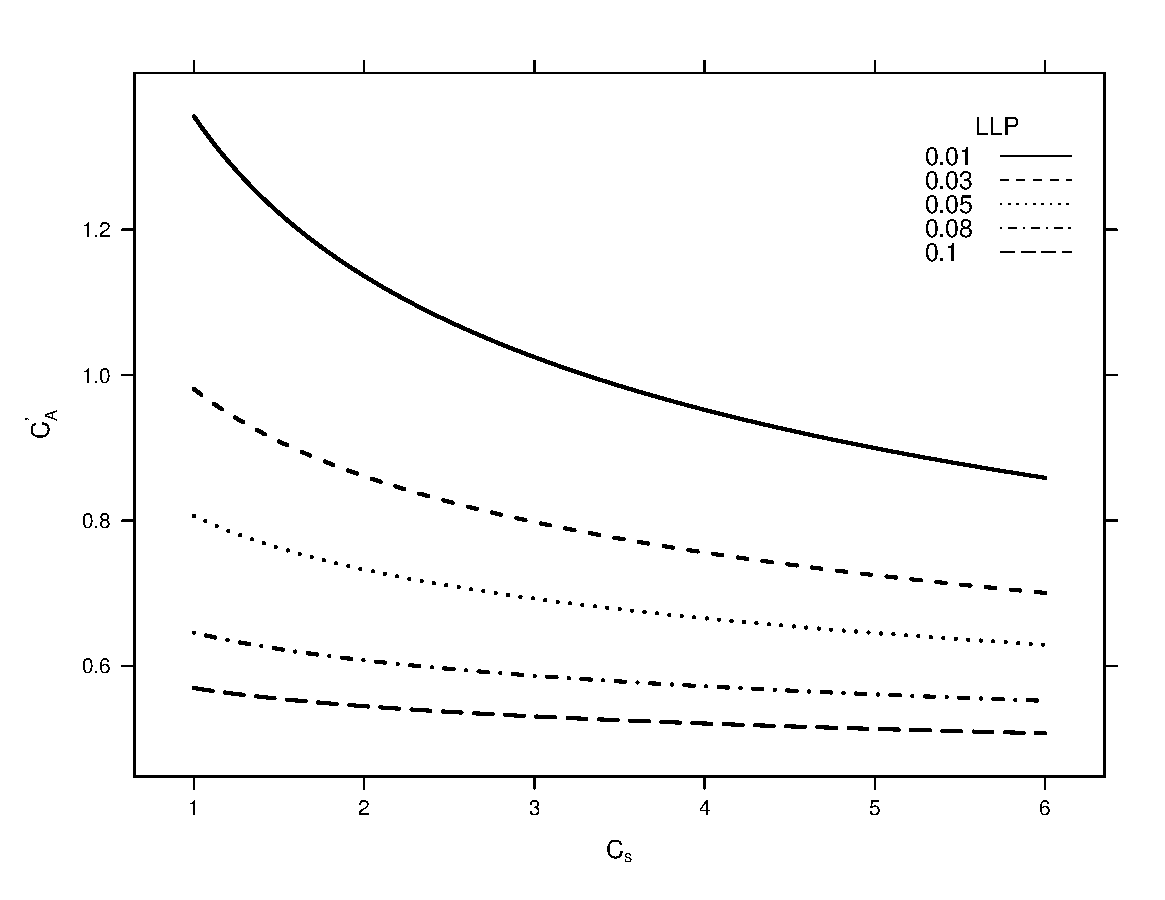
\includegraphics[scale=0.75]{../figs/CurvasLLP}

\caption{Curvas LLP.\label{fig:Curvas-LLP}}



\end{figure}


%
\begin{figure}
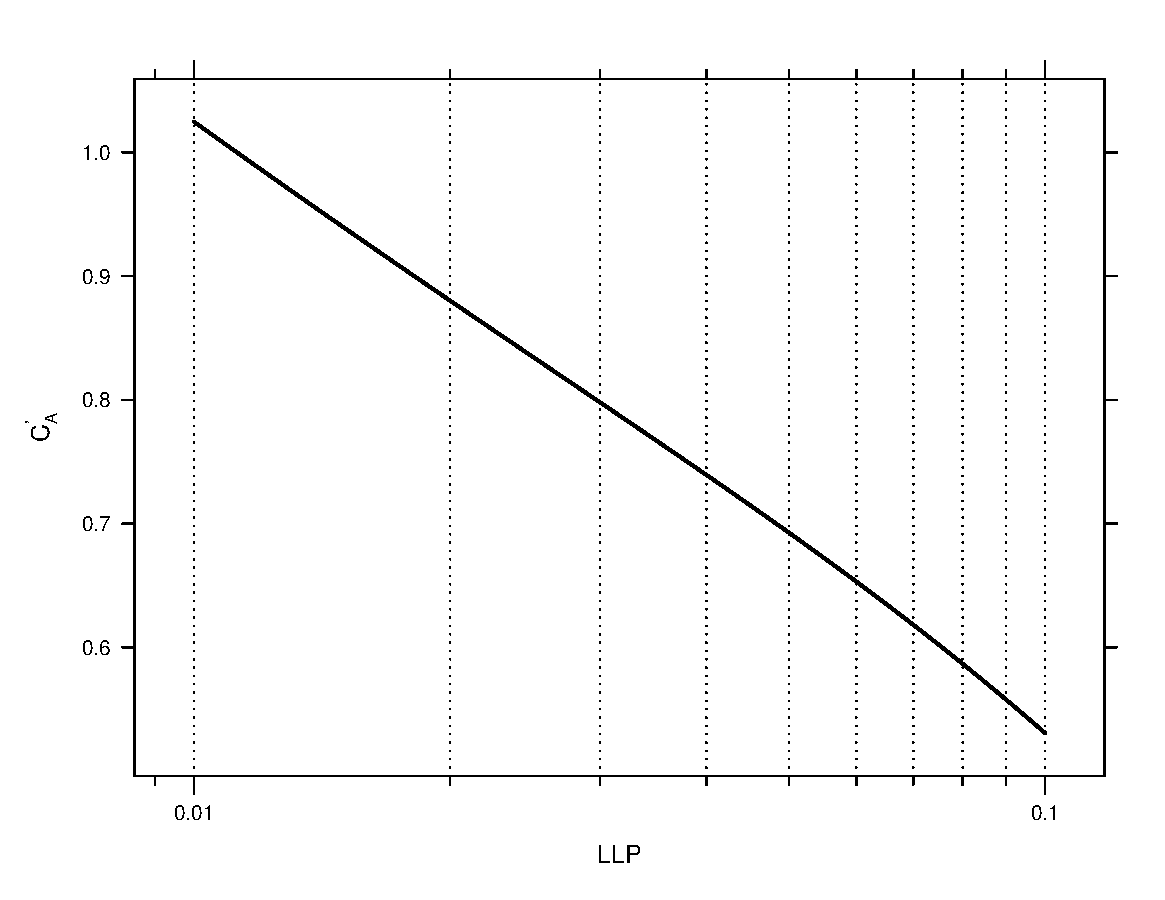
\includegraphics[scale=0.75]{../figs/CurvasLLP_Cs3}

\caption[Relación entre $C_{A}^{'}$ y LLP]{Relación entre $C_{A}^{'}$ y LLP para $C_{S}=3$ (escala logarítmica
en LLP).\label{fig:Ca_LLP_Cs3}}

\end{figure}



\subsubsection{Métodos basados en la experiencia}

En base a los sistemas instalados y en funcionamiento, es posible
establecer valores de $C_{A}$ y $C_{S}$ que se adaptan bien a las
aplicaciones más comunes, sin llevar a cabo el cálculo detallado del
funcionamiento del sistema. La ventaja evidente de este método es
la sencillez, si bien como contrapartida no permite establecer análisis
de fiabilidad. En la actualidad, esta aproximación al dimensionado
del sistema es, con diferencia, la más empleada en las licitaciones
de electrificación rural fotovoltaica.

Según la Norma Técnica Universal \citep{Egido.Lorenzo1998} los valores
recomendados para sistemas domésticos son $C_{A}=1.1$ y $3\leq C_{S}\leq5$,
mientras que para aplicaciones profesionales son $1.2\leq C_{A}\leq1.3$
y $5\leq C_{S}\leq8$. Estos valores de utilización general pueden
ser sustituidos en el caso de España por los recogidos en la Tabla
\ref{tab:ValoresCACSEspana}.

%
\begin{table}
\caption[Valores recomendados de capacidad del generador y capacidad del acumulador
aplicables a SFA en España.]{Valores recomendados de capacidad del generador $C_{A}$ y capacidad
del acumulador $C_{S}$ aplicables a SFA en España \citep{Lorenzo2006c}.\label{tab:ValoresCACSEspana}}


\centering{}\begin{tabular}{ccccc}
\toprule 
 & \multicolumn{4}{c}{Aplicación}\tabularnewline
\cmidrule{2-5} 
 & \multicolumn{2}{c}{Doméstica} & \multicolumn{2}{c}{Profesional}\tabularnewline
\midrule
\midrule 
Zona & $C_{A}$ & $C_{S}$ & $C_{A}$ & $C_{S}$\tabularnewline
\midrule 
Norte de España & 1,2 & 5 & 1,3 & 8\tabularnewline
\midrule 
Sur de España & 1,1 & 4 & 1,2 & 6\tabularnewline
\bottomrule
\end{tabular}
\end{table}



\subsection{Configuración de generador y acumulador}

Una vez elegidos los valores de $C_{A}$ y $C_{S}$, se deben configurar
el generador y batería de acuerdo a las tensiones de trabajo. Recordemos
que es la batería la que impone la tensión de trabajo. Normalmente
los SFA no incorporan buscador de MPP como es común en los sistemas
fotovoltaicos conectados a red, aunque es posible configurar la batería
y el generador para que la tensión de la batería, $V_{b}$, esté cerca
del MPP, $V_{mpp}$ (considerando la influencia de la temperatura).
En base a la tensión de la batería obtenemos las ecuaciones \ref{eq:L_Tension}
y \ref{eq:TamanoGenerador_Tension}:

\begin{eqnarray}
L & = & V_{b}\cdot Q_{L}\label{eq:L_Tension}\\
\eta_{G}\cdot A_{G}\cdot G_{stc} & = & I_{g}^{*}\cdot V_{b}\label{eq:TamanoGenerador_Tension}\end{eqnarray}
donde $\eta_{G}$ incluye las pérdidas debidas a la temperatura de
funcionamiento, y de ahí que consideremos que $V_{mpp}\simeq V_{b}$.
A partir de las ecuaciones \ref{eq:CA} y \ref{eq:Cs} se obtienen
las ecuaciones \ref{eq:CorrienteCA} y \ref{eq:QbCs}: 

\begin{eqnarray}
I_{g}^{*} & = & \frac{C_{A}\cdot Q_{L}\cdot G_{stc}}{\overline{G_{d}}(\beta,\alpha)}\label{eq:CorrienteCA}\\
C_{U} & = & C_{S}\cdot Q_{L}\label{eq:QbCs}\end{eqnarray}
\nomenclature[Ql]{$Q_{L}$}{Carga demandada en amperios-hora}siendo
$I_{g}^{*}$ la corriente del generador en el punto MPP en condiciones
STC%
\footnote{En este punto estamos despreciando las pérdidas debidas a la temperatura.
Esta aproximación es asumible teniendo en cuenta que, a la hora de
configurar eléctricamente el generador, los valores discretos de tensión
y corriente de módulos disponibles en el mercado conducen a tamaños
de generador mayor de lo que resulta de la ecuación \ref{eq:TamanoGenerador_Tension}%
}, $Q_{L}$ la carga a satisfacer en amperios-hora, y $C_{U}$ la capacidad
útil de la batería en amperios-hora. Al elegir el regulador, su tensión
de funcionamiento deberá estar en consonancia con la del sistema.
Se recomienda que su corriente máxima sea un $\SI{20}{\percent}$
superior a la de funcionamiento del sistema.

No todos los valores de tensión de batería están disponibles en el
mercado. Los vasos tienen una tensión nominal de $\SI{2}{\volt}$,
y las baterías comerciales son agrupaciones serie de vasos para ofrecer
tensiones nominales de $\SI{12}{\volt}$, $\SI{24}{\volt}$ y $\SI{48}{\volt}$.
Lo mismo sucede con los valores de capacidad de batería y corriente
del generador. Por esta razón, al elegir equipos que se adapten a
los resultados de las ecuaciones \ref{eq:CorrienteCA} y \ref{eq:QbCs},
generalmente sobredimensionaremos ligeramente el generador, la batería
o ambos para que la configuración eléctrica se adecue al dimensionado
del sistema. Dado que los resultados de las ecuaciones \ref{eq:CorrienteCA}
y \ref{eq:QbCs} corresponden a equipos nuevos y en condiciones nominales,
en algunos casos puede ser conveniente incorporar un factor de seguridad
para tener en cuenta la disminución de la capacidad asociada al envejecimiento.

La evolución de los elementos que componen el acumulador no es homogénea
y aparecerán diferencias que se acentuarán con el tiempo. Esta dispersión
de características es dañina porque el regulador impondrá las mismas
condiciones de trabajo a todos los elementos, de forma que aquellos
menos robustos alcanzarán su fin de vida útil de forma más precipitada
que si no hubieran formado parte de la agrupación. Cuando el acumulador
está compuesto por elementos en serie, estos problemas pueden ser
solventados en gran medida con sobrecargas controladas para homogeneizar
el conjunto. Esta técnica no soluciona el problema cuando la agrupación
incluye conexiones de vasos en paralelo. Por esta razón, la Norma
Técnica Universal marca como obligatorio evitar la conexión en paralelo
de más de dos baterías y en todo caso debe impedirse la conexión en
paralelo de dos baterías diferentes o una batería nueva con una vieja.


\subsection{Orientación e inclinación del generador}

Como se estudió en la sección correspondiente de los sistemas de conexión
a red (sección \ref{sub:Orientacion-e-inclinacion}),
el generador fotovoltaico deberá contar con una orientación e inclinación
particularmente adaptadas al lugar y a la aplicación. Nuevamente,
la orientación siempre será hacia el Sur en el hemisferio Norte y
hacia el Norte en el hemisferio Sur. Sin embargo, la inclinación depende
ahora, no sólo de la latitud sino también del perfil del consumo.
Así, para instalaciones con consumos constantes o similares a lo largo
del año, el objetivo es maximizar la radiación en los meses de menor
insolación y por tanto la inclinación debe ser $\beta=|\phi|+10^{\circ}$.
Para instalaciones con consumo menor en los meses de baja radiación
se busca maximizar la radiación en los equinoccios y de ahí que $\beta=|\phi|$.
Finalmente, para instalaciones con uso predominante en verano conviene
emplear un ángulo inferior a la latitud, $\beta=|\phi|-10^{\circ}$.
En general, la inclinación debe superar los $15^{\circ}$para conseguir
que la lluvia pueda desplazar la suciedad acumulada en los paneles.


\subsection{Cálculo del consumo\label{sub:Estimacion-del-consumo}}

Las cargas conectadas a un SFA pueden ser de corriente continúa y
corriente alterna. Suponiendo conocida la energía requerida por cada
grupo de cargas (o de forma equivalente, su potencia nominal y horas
típicas de uso), la energía total, $L_{T}$, que debe entregar el
SFA viene dada por la ecuación \ref{eq:EnergiaConsumoPerdidas}\begin{equation}
L_{T}=\frac{L_{dc}}{\eta_{r}}+\frac{L_{ac}}{\eta_{inv}}\label{eq:EnergiaConsumoPerdidas}\end{equation}
siendo $L_{dc}$ la energía debida a las cargas de corriente continua,
$L_{ac}$ la debida a las cargas de corriente alterna, y $\eta_{r}$
y $\eta_{inv}$\nomenclature[Lt]{$L_{T}$}{Energía total requerida a un sistema autónomo, incluyendo pérdidas de los elementos}\nomenclature[Ldc]{$L_{dc}$}{Energía de las cargas de corriente continua en un sistema autónomo}\nomenclature[etar]{$\eta_{r}$}{Rendimiento del regulador de un sistema autónomo}\nomenclature[etab]{$\eta_{bat}$}{Rendimiento energético de un acumulador electroquímico}\nomenclature[etac]{$\eta_{c}$}{Rendimiento energético del cableado}
los rendimientos energéticos del regulador y el inversor, respectivamente.
Parte de la energía producida por el generador fotovoltaico llega
a las cargas después de haber sido transformada en la batería. Ya
vimos que la eficiencia de transformación de la batería dependía de
su estado de carga, alcanzando valores bajos al acercarse al fin de
carga. Dicho de otra forma, parte de la energía que produce el generador
fotovoltaico no llegará a las cargas, pero debe ser tenida en cuenta
en el cálculo como una pérdida más. Utilizaremos un rendimiento promedio,
$\eta_{bat}$, que tendrá en cuenta la eficiencia de la batería en
los diferentes estados de carga y el porcentaje de energía que transita
directamente entre el generador y las cargas sin atravesar la batería.
Otras pérdidas que deben ser tenidas en cuenta son las debidas al
efecto Joule en los cables, $\eta_{c}$. Por tanto, el valor final
de $L$ resulta de la ecuación \ref{eq:EnergiaConsumoFinal}:\begin{equation}
L=\frac{L_{T}}{\eta_{bat}\cdot\eta_{c}}\label{eq:EnergiaConsumoFinal}\end{equation}
\nomenclature[Ltotal]{L}{Energía total requerida a un sistema autónomo, incluyendo pérdidas de los elementos}

Como valores orientativos pueden utilizarse $\eta_{inv}=0.9$, $\eta_{r}=0.95$,
$\eta_{bat}=0.85$ y $\eta_{c}=0.98$.

Hasta aquí hemos considerado conocido el consumo requerido por las
cargas conectadas al SFA. Sin embargo, el carácter aleatorio del comportamiento
humano dificulta la caracterización del consumo eléctrico. Recogemos
aquí las palabras de dos investigadores brasileños \citep{Morante.Zilles2008}:
\begin{quotation}
{}``{[}...{]} teóricamente, en una sociedad igualitaria la representación
gráfica del consumo eléctrico debiera seguir la forma de una distribución
Normal. Obviamente, en este caso {[}...{]} la mayoría de las familias
mostrarían un consumo cercano a la media. Sin embargo, no es esto
lo que ocurre, sino que en la realidad este comportamiento se corresponde
con una distribución Gamma. En palabras sencillas, lo que esta función
y sus parámetros relacionados expresan es que 'mucha gente consume
poco y poca gente consume mucho'. Este hecho se debe a la interrelación
de una serie de factores técnicos, de gestión, psicológicos, geográficos,
demográficos, socioculturas y económicos. Todos ellos, dependiendo
del grado de predominancia de cada uno, con mayor o menor intensidad
definen el nivel de consumo eléctrico de cada familia.''
\end{quotation}
Como ejemplo, en la figura \ref{fig:Distribucion-de-probabilidades}
se recoge la modelización del consumo eléctrico mensual de las poblaciones
brasileñas analizadas en la citada referencia. Es destacable cómo
tanto la distribución de probabilidad como el valor medio dependen
de la localidad. 

%
\begin{figure}
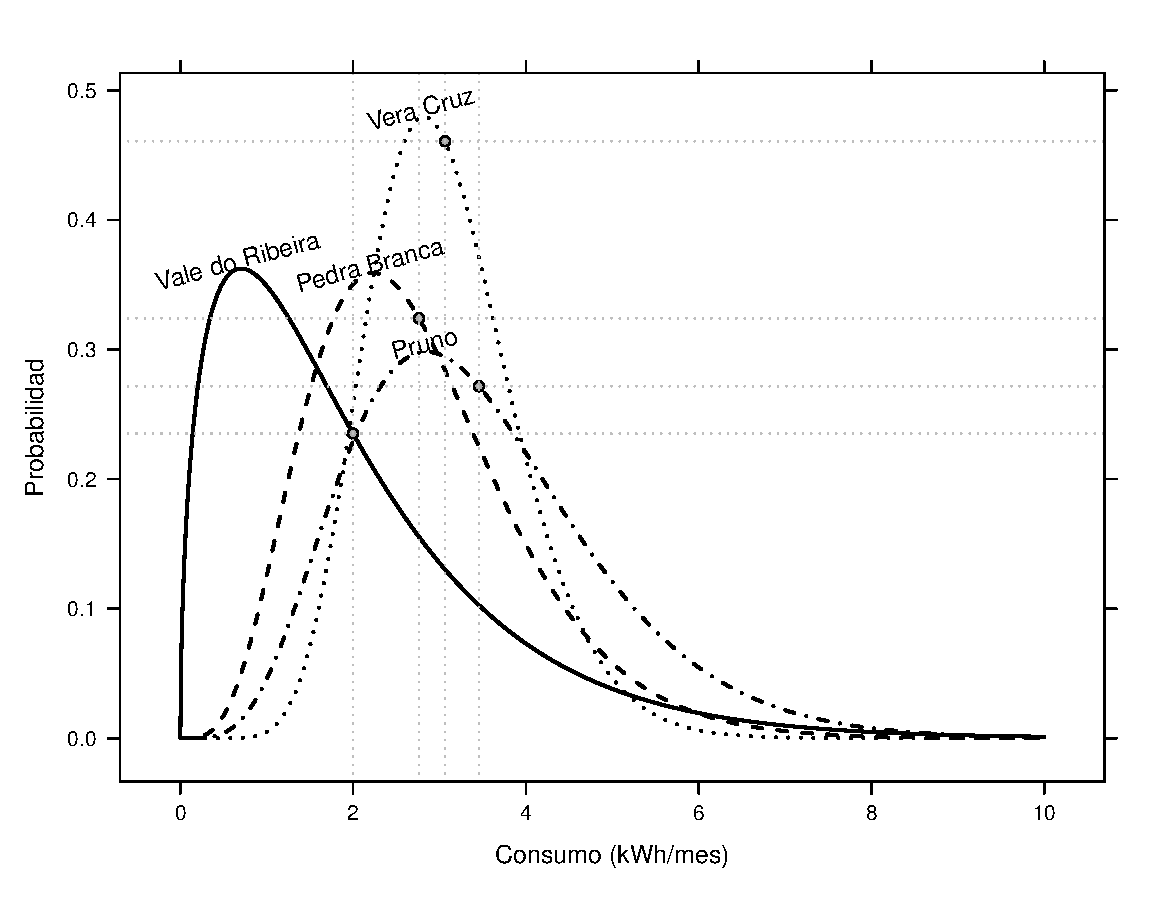
\includegraphics[scale=0.6]{../figs/ConsumoGamma}

\caption[Distribución de probabilidades del consumo mensual en cuatro localidades
brasileñas]{\label{fig:Distribucion-de-probabilidades}Distribución de probabilidades
del consumo mensual en cuatro localidades brasileñas analizadas en
\citep{Morante.Zilles2008}. Se señala el valor medio de consumo en
cada una las curvas. }



\end{figure}


A la hora de dimensionar el sistema, será necesario adoptar un conjunto
pequeño de valores estándar aplicables a diferentes grupos de consumo
indentificables con las curvas mostradas. Con este conjunto de valores
estándar de consumo se lleva a cabo el proceso de dimensionamiento
de varios SFA correspondientes a cada grupo. Esta estandarización
es necesaria para conseguir reducir costes, para facilitar la gestión
de la logística y la instalación, y para poder prestar un servicio
de mantenimiento eficiente. Sin embargo, al tratar a todos los usuarios
de un mismo grupo como si su consumo fuese idéntico se obtendrán SFA
cuya fiabilidad no será la de diseño. En la figura \ref{fig:ConsumoLLP}
se analiza esta situación \citep{Lorenzo.Narvarte2000}. En primer
lugar se calcula el tamaño de un generador y una batería para satisfacer
un determinado consumo, $L_{base}$, con una fiabilidad determinada,
$LLP_{base}$. Con los resultados de este caso base, manteniendo invariables
el tamaño del generador y batería, se calcula la fiabilidad que corresponde
a consumos diferentes a los del caso base. La curva que relaciona
el ratio $\frac{LLP}{LLP_{base}}$ con $\frac{L}{L_{base}}$
muestra, por ejemplo, cómo una variación del 60\% en el consumo implica
disminuir a la mitad la fiabilidad del sistema. De aquí se concluye
que empeñarse en un ejercicio de dimensionado de gran precisión carece
de demasiada utilidad. Más importante resulta emplear los métodos
reseñados para tomar las decisiones oportunas que garanticen el buen
funcionamiento del sistema elegido en un amplio abanico de condiciones
de funcionamiento, tanto ambientales como humanas.

%
\begin{figure}
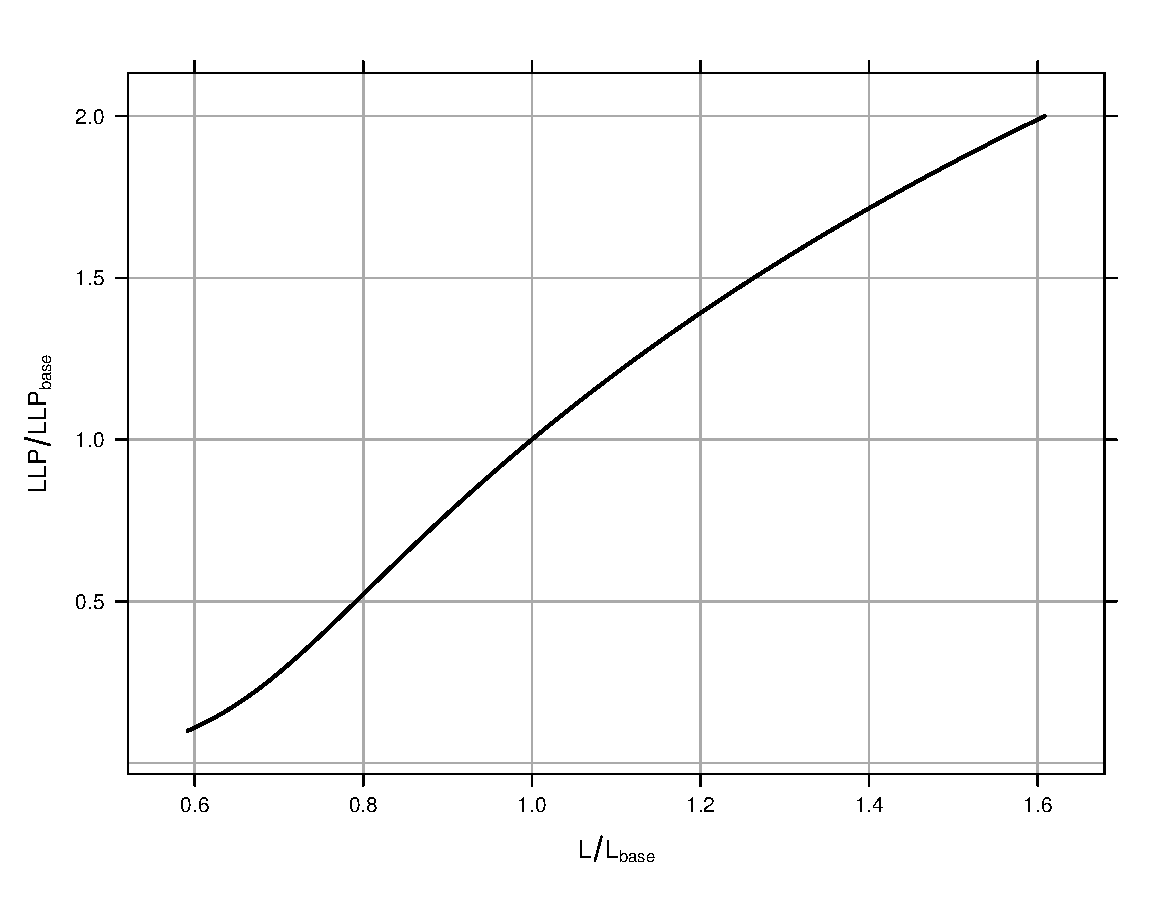
\includegraphics[scale=0.6]{../figs/ConsumoLLP}

\caption{Relación entre el consumo y la fiabilidad cuando se mantienen invariables
el tamaño de un generador y una batería dimensionados para satisfacer
un consumo $L_{base}$ con una $LLP_{base}$.\label{fig:ConsumoLLP}}



\end{figure}


Aún así, y con la debida cautela derivada de los comentarios anteriores,
es útil establecer unos escenarios de consumo que sirvan de orientación
para los primeros cálculos. Quedan recogidos en la tabla \ref{tab:Escenarios-de-consumo}. 

Cerramos este capítulo recomendando la referencia \citep{IngenieriaSinFronteras1999}
al lector interesado en los aspectos sociológicos de la comunidad
receptora que influyen en el diseño, implantación y mantenimiento
de un sistema fotovoltaico.

%
\begin{table}
\caption[Escenarios de consumo para SFA.]{Escenarios de consumo para SFA \citep{Lorenzo2006c}.\label{tab:Escenarios-de-consumo}}


\begin{tabular}{>{\centering}p{2cm}>{\centering}p{6cm}>{\centering}p{3cm}}
\toprule 
Aplicación & Hipótesis de consumo & Criterio de dimensionado\tabularnewline
\midrule
\midrule 
SHS1 & \begin{itemize}
\item Iluminación
\item Radio 
\item TV b/n
\item Sin frigorífico
\item 120 Wh/día
\end{itemize}
 & \begin{eqnarray*}
C_{A} & = & 1.1\\
3\leq & C_{s} & \leq5\end{eqnarray*}
\tabularnewline
\midrule 
SHS2 & \begin{itemize}
\item Iluminación
\item Radio
\item TV color
\item Sin frigorífico
\item 250 Wh/día
\end{itemize}
 & \begin{eqnarray*}
C_{A} & = & 1.1\\
3\leq & C_{s} & \leq5\end{eqnarray*}
\tabularnewline
\midrule 
SHS3 & \begin{itemize}
\item Iluminación
\item radio
\item TV color
\item Con frigorífico eficiente
\item 1000 Wh/día
\end{itemize}
 & \begin{eqnarray*}
C_{A} & = & 1.1\\
C_{S} & = & 5\end{eqnarray*}
\tabularnewline
\midrule 
Centrales & \begin{itemize}
\item Todo AC 
\item 500 Wh/día por vivienda
\end{itemize}
 & \begin{eqnarray*}
C_{A} & = & 1.1\\
C_{S} & = & 5\end{eqnarray*}
\tabularnewline
\end{tabular}
\end{table}

%%% Local Variables:
%%% mode: LaTex
%%% TeX-master: "ESF.tex"
%%% End: 